\chapter*{graphics}\addcontentsline{toc}{chapter}{graphics}

\HCode{<hr>}
Drawing functions
\begin{quote}
\noindent
\hyperlink{Matplot}{Matplot} - 2D plot of a matrix using colors\\
\hyperlink{Matplot1}{Matplot1} - 2D plot of a matrix using colors \\
\hyperlink{Sgrayplot}{Sgrayplot} - 2D plot of a surface using colors \\
\hyperlink{Sfgrayplot}{Sfgrayplot} - 2D plot of a surface using colors \\
\hyperlink{bode}{Bode plot}\\
\hyperlink{champ}{champ} - 2D vector field plot \\
\hyperlink{champ1}{champ1} - 2D vector field plot \\
\hyperlink{colormap}{colormap} - using colormaps in graphics\\
\hyperlink{contour2di}{contour2di} - compute points of level curves of a surface\\
\hyperlink{contour2d}{contour2d} - level curves of a surface on a 2 dimensional plot\\
\hyperlink{contourf}{contourf}  - level curves of a surface on a 2 dimensional plot\\
\hyperlink{contour}{contour}  - level curves of a surface on a 3 dimensional plot\\
\hyperlink{evans}{evans} - Evans root locus\\
\hyperlink{fec}{fec} -  plot of a function defined on a triangular mesh\\
\hyperlink{graycolormap}{graycolormap} - linear gray colormap from black to white\\
\hyperlink{grayplot}{grayplot} - 2D plot of a surface using colors \\
\hyperlink{greencolormap}{greencolormap} - linear green colormap\\
\hyperlink{histplot}{histplot} - draw an histogram of the components of a vector of numbers\\
\hyperlink{hotcolormap}{hotcolormap} - red to yellow colormap\\
\hyperlink{jetcolormap}{jetcolormap} - blue to red colormap \\
\hyperlink{nyquist}{nyquist plot}\\
\hyperlink{param3d}{param3d} - 3D plot of a parametric curve\\
\hyperlink{param3d1}{param3d1} - 3D plot of a parametric curve\\
\hyperlink{plot2d}{plot2d} - draw two dimensional graphs\\
\hyperlink{plot3d}{plot3d} - 3D plot of a surface \\
\hyperlink{polarplot}{polarplot} - draw a curve given with polar coordinates \\
\hyperlink{subplot}{subplot} - graphic sub windows specification\\
\hyperlink{winsid}{winsid} - graphics windows ids\\
\hyperlink{xarcs}{xarcs} - draw parts of a set of ellipses \\
\hyperlink{xarc}{xarc} - draw a part of an ellipse\\
\hyperlink{xarrows}{xarrows} - draw a set of arrows \\
\hyperlink{xclear}{xclear} - clears a graphics window \\
\hyperlink{xdel}{xdel} - delete a graphics window \\
\hyperlink{xexport}{export graphics to a file}\\
\hyperlink{xfarcs}{xfarcs} - fill parts of a set of ellipses \\
\hyperlink{xfarc}{xfarc} - fill part of an ellipse\\
\hyperlink{xfpolys}{xfpolys} - fill a set of polygons \\
\hyperlink{xfpoly}{xfpoly} - fill a polygon with color \\
\hyperlink{xfrect}{xfrect} - fill a rectangle \\
\hyperlink{xpolys}{xpolys} - draw a set of polylines or polygons \\
\hyperlink{xpoly}{xpoly} - draw a polyline or a polygon \\
\hyperlink{xrects}{xrects} - draw a set of rectangles\\
\hyperlink{xrect}{xrect} - draw a rectangle\\
\hyperlink{xsegs}{xsegs} - draw unconnected segments \\
\hyperlink{xselect}{xselect} - raise the current graphic window\\
\hyperlink{xsetech}{xsetech} - set parameters of a subwindow in a graphic window\\
\hyperlink{xstringl}{xstringl} - enclosing rectangle when drawing a string matrix \\
\hyperlink{xstring}{xstring} - draw a string matrix \\
\hyperlink{xtitle}{xtitle} - sets the main title and the axis labels of a graph\\
\end{quote}

\HCode{<hr>}
Dealing with surfaces data
\begin{quote}
\noindent
\hyperlink{eval3d}{eval3d} - evaluates a function on a grid \\
\hyperlink{eval3dp}{eval3dp} - compute facets for a 3D parametric surface\\
\hyperlink{genfac3d}{genfac3d} - compute facets of a 3D surface\\
\hyperlink{nf3d}{nf3d} - build rectangular facets adapted to plot3d \\
\end{quote}

% -*- mode: latex -*-

\mansection{Matplot}
\begin{mandesc}
  \short{Matplot}{2D plot of a matrix using colors}\\
  \short{Matplot1}{2D plot of a matrix using colors}\\
\end{mandesc}
%-- Calling sequence section
\begin{calling_sequence}
\begin{verbatim}
  Matplot(M,options=values)
  Matplot1(M,mrect,options=values)
\end{verbatim}
\end{calling_sequence}

%-- Parameters
\begin{parameters}
  \begin{varlist}
    \vname{M}: real matrix of size (n1,n2).
    \vname{mrect}: rectangle \verb![xmin,ymin,xmax,ymax]! giving the position where the matrix display must be inserted.
    \vname{remap}: if true then the values in \verb!M! are mapped to colors
    \vname{zminmax}: gives the range of values which must be remapped to colors (default value is
    \verb![min(M),max(M)]!.
    \vname{colminmax}: gives the range of colors to which \verb!zminmax! values are to be mapped
    (default value is \verb![1,xget('lastpattern')]! i.e all the available colors in the current
    colormap).
    \vname{axesflag}: see \manlink{plot2d}{plot2d}
    \vname{frameflag}: see \manlink{plot2d}{plot2d}
    \vname{leg}:  see \manlink{plot2d}{plot2d}
    \vname{leg_pos}:  see \manlink{plot2d}{plot2d}
    \vname{logflag}:  see \manlink{plot2d}{plot2d}
    \vname{nax}: see \manlink{plot2d}{plot2d}
    \vname{rect}:  see \manlink{plot2d}{plot2d}
    \vname{auto_axis}:  see \manlink{plot2d}{plot2d}
    \vname{iso}:  see \manlink{plot2d}{plot2d}
  \end{varlist}
\end{parameters}

\begin{mandescription}
  \verb!Matplot! display matrix values as colored squares remapping values to colormap entries
  if \verb!remap=%t! or using matrix values as color entries in current colormap
  if \verb!remap=%f!.

  When using \verb!Matplot1!, the second argument gives the rectangle coordinates
  where the matrix is to be displayed.
\end{mandescription}

%--example
\begin{examples}

\noindent A simple example

\begin{mintednsp}{nsp}
  xset('colormap',jetcolormap(100));
  Matplot(testmatrix('magic',10))
\end{mintednsp}

\noindent Vizualize the current colormap

\begin{mintednsp}{nsp}
  Matplot((1:xget("lastpattern")))
\end{mintednsp}

\noindent An example with \verb!Matplot1!.

\begin{mintednsp}{nsp}
  N=32;
  C=[jetcolormap(N);graycolormap(N);hotcolormap(N)];
  xset('colormap',C);
  M=[1:N;N+(1:N);2*N+(1:N)];
  Matplot1(M,[1,1,32,3],rect=[-10,1,32,3],axesflag=2);
  xstring(-8,1.4,'hotcolormap');
  xstring(-8,2.0,'graycolormap');
  xstring(-8,2.6,'jetcolormap');
\end{mintednsp}

\noindent An example with remap

\begin{mintednsp}{nsp}
  N=32;C=[jetcolormap(N)]; xset('colormap',C);
  Matplot(1:32,remap=%t,zminmax=[10,20],colminmax=[20,32]);
\end{mintednsp}
\end{examples}
%-- see also
\begin{manseealso}
  \manlink{colormap}{colormap}
  \manlink{plot2d}{plot2d}
  \manlink{Matplot1}{Matplot1}
\end{manseealso}
%-- Author
\begin{authors}
  J.-Ph. C.
\end{authors}

% -*- mode: latex -*-
\mansection{Sgrayplot}
\begin{mandesc}
  \short{Sgrayplot}{smooth 2D plot of a surface using colors}\\
  \short{Sfgrayplot}{smooth 2D plot of a surface using colors}\\
\end{mandesc}
%-- Calling sequence section
\begin{calling_sequence}
\begin{verbatim}
  Sgrayplot(x,y,z,options=value)
  Sfgrayplot(x,y,f,options=value)
\end{verbatim}
\end{calling_sequence}
%-- Parameters
\begin{parameters}
  \begin{varlist}
    \vname{x,y}: real row vectors of size \verb!n1! and \verb!n2!.
    \vname{z}: real matrix of size \verb!n1xn2!.
    The z-value of the surface at \verb!(x(i),y(j))! is given by \verb!z(i,j)!
    \vname{f}: a nsp function. The z-value of the surface at point \verb!(x(i),y(j))!
    is given by \verb!f(x(i),y(j))!
    \vname{options=value}: a sequence of optional names values (See \manlink{fec}{fec}).
  \end{varlist}
\end{parameters}

\begin{mandescription}
  \verb!Sgrayplot! is similar to \verb!grayplot! but the plot is done using the
  \verb!fec! function. The surface is plotted assuming that it is linear on a set of
  triangles built from the grid (here with n1=5, n2=3):
  \begin{Verbatim}
    _____________
    | /| /| /| /|
    |/_|/_|/_|/_|
    | /| /| /| /|
    |/_|/_|/_|/_|
  \end{Verbatim}
  Optional parameters are described in the manual page of function \manlink{fec}{fec}.
\end{mandescription}

%--example
\begin{examples}
\noindent A first example
  \begin{mintednsp}{nsp}
    xclear();
    x=-10:10; y=-10:10;m =rand(21,21);
    xset("colormap",hotcolormap(64))
    Sgrayplot(x,y,m, colorbar=%t);
  \end{mintednsp}

\noindent A second example

  \begin{mintednsp}{nsp}
    xclear();
    n = 30;
    nt = 100;
    x = linspace(0,2*%pi,n);
    y = linspace(0,%pi,n/2);
    z = sin(x')*sin(y);
    t = linspace(0,4*%pi,nt);
    xset("colormap",jetcolormap(64));
    Sgrayplot(x,y,cos(t(1))*z, colorbar=%t);
    F=get_current_figure[];
    fecd=F.children(1).children(1);
    for i=1:nt
      fecd.func = cos(t(i))*z;
      fecd.invalidate[];
      xpause(10000,%t);
    end
  \end{mintednsp}

  \noindent Using functions for describing surfaces

  \begin{mintednsp}{nsp}
    xclear();
    function z=surf1(x,y), z=x*y, endfunction
    function z=surf2(x,y), z=x^2-y^2, endfunction
    function z=surf3(x,y), z=x^3+y^2, endfunction
    function z=surf4(x,y), z=x^2+y^2, endfunction
    xset("colormap",[jetcolormap(64);hotcolormap(64)])
    x = linspace(-1,1,60);
    y = linspace(-1,1,60);
    subplot(2,2,1)
    Sfgrayplot(x,y,surf1,axesflag=0,colorbar=%t,colminmax=[1,64]);
    xtitle("f(x,y) = x*y")
    subplot(2,2,2)
    Sfgrayplot(x,y,surf2,axesflag=0,colorbar=%t,colminmax=[65,128])
    xtitle("f(x,y) = x^2-y^2")
    subplot(2,2,3)
    Sfgrayplot(x,y,surf3,axesflag=0,colorbar=%t,colminmax=[65,128])
    xtitle("f(x,y) = x^3+y^2")
    subplot(2,2,4)
    Sfgrayplot(x,y,surf4,axesflag=0,colorbar=%t,colminmax=[1,64])
    xtitle("f(x,y) = x^2+y^2")
  \end{mintednsp}

  % \noindent Adding some level curves
  % \begin{nspcode}
  %   function z=surf3(x,y), z=x^3+y^2, endfunction
  %   x = linspace(-1,1,60);
  %   y = linspace(-1,1,60);
  %   xset("colormap",hotcolormap(128))
  %   Sfgrayplot(x,y,surf3,strf="041")
  %   fcontour2d(x,y,surf3,rect=[-0.1, 0.025, 0.4],style=[1 1 1],strf="000")
  %   xtitle("f(x,y) = x^3+y^2")
  % \end{nspcode}

\end{examples}
%-- see also
\begin{manseealso}
  \manlink{fec}{fec}
  \manlink{fgrayplot}{fgrayplot}
  \manlink{grayplot}{grayplot}
\end{manseealso}
%-- Author

% -*- mode: latex -*-
\mansection{bode}
\begin{mandesc}
  \short{bode}{Bode plot}\\
\end{mandesc}
%-- Calling sequence section
\begin{calling_sequence}
\begin{verbatim}
  bode(n,d,fmin=,fmax=,step=,frq=,title=,dom=)
\end{verbatim}
\end{calling_sequence}
%-- Parameters
\begin{parameters}
  \begin{varlist}
    \vname{n,d}: two polynomial matrices of size \verb!nx1!
    \vname{fmin}: a real for minimal frequency bounds (in Hz) or \verb!sym!
    \vname{fmax}: a real for maximal frequency bounds (in Hz).
    \vname{step}: a real (logarithmic step) or a string \verb!'auto'!.
    \vname{title}: a \verb!nx1! string matrix (captions for each curve).
    \vname{frq}: a row vector or a \verb!nx1! matrix giving frequencies (in Hz).
    \vname{dom}: time domain \verb!'c'! or \verb!'d'! or a positive real (default \verb!'c'!).
  \end{varlist}
\end{parameters}

\begin{mandescription}
  Bode plot, i.e magnitude and phase of the frequency response of the system
  \verb!n/d!. The system can be a continuous-time (\verb!dom='c'!) or
  discrete-time (\verb!dom='d'! or a positive real) SIMO system.

  The frequencies are given by the matrix \verb!frq! or computed from
  the bounds \verb!fmin! and \verb!fmax! (in Hz) and \verb!step! giving
  the ( logarithmic ) discretization step which is automatically adapted if
  (\verb!step='auto'!).
\end{mandescription}

%--example
\begin{examples}
  \begin{mintednsp}{nsp}
    s=poly(0,'s')
    n=(s^2+2*0.9*10*s+100);d=(s^2+2*0.3*10.1*s+102.01);
    n1=n*(s^2+2*0.1*15.1*s+228.01); d1=d*(s^2+2*0.9*15*s+225);
    bode([n;n1],[d;d1],fmin=0.01,fmax=100,title=['h1';'h'])
  \end{mintednsp}
\end{examples}

%-- see also
\begin{manseealso}
  \manlink{nyquist}{nyquist}
  \manlink{gainplot}{gainplot}
  %\manlink{black}{black}
  %\manlink{repfreq}{repfreq}
  %\manlink{g\_margin}{g-margin}
  %\manlink{p\_margin}{p-margin}
  %\manlink{calfrq}{calfrq}
  %\manlink{phasemag}{phasemag}
\end{manseealso}

% -*- mode: latex -*-
\mansection{champ}
\begin{mandesc}
  \short{champ}{2D vector field plot}\\ % @mandesc@
  \short{champ1}{2D vector field plot}\\ % @mandesc@
\end{mandesc}
%-- Calling sequence section
\begin{calling_sequence}
\begin{verbatim}
  champ(x,y,fx,fy,arfact=,rect=,strf=)
  champ1(x,y,fx,fy,arfact=,rect=,strf=)
\end{verbatim}
\end{calling_sequence}
%-- Parameters
\begin{parameters}
  \begin{varlist}
    \vname{x,y}: two vectors which define the grid points
    \vname{fx,fy}: two matrices which describes the x and y component of the vector field.
    \vname{arfact}: an optional argument of type real which gives a scale factor
    for the drawing of the arrows head (default value is 1.0)
    \vname{rect}: a vector \verb!rect=[xmin,ymin,xmax,ymax]! which gives
    the boundaries of the graphics frame to use.
    \vname{strf}: a string of length 3 "xyz" which has the same meaning as the
    \verb!strf! parameter of \verb!plot2d!. The first
    character x has no effect with \verb!champ!.
  \end{varlist}
\end{parameters}

\begin{mandescription}
  The functions \verb!champ! and \verb!champ1! are used to draw two dimensional
  vector fields. When using \verb!champ!, the length of the arrows is proportional to the intensity of the field.
  When using \verb!champ1! the color id used to draw the arrow is proportional to the intensity of the field.
\end{mandescription}
%--example
\begin{examples}

  \noindent A simple example with \verb!champ!
  \begin{mintednsp}{nsp}
    champ(-5:5,-5:5,rand(11,11),rand(11,11));
  \end{mintednsp}
  \noindent A simple example with \verb!champ1!
  \begin{mintednsp}{nsp}
    champ1(-5:5,-5:5,rand(11,11),rand(11,11),arfact=2,rect=[-10,-10,10,10]);
  \end{mintednsp}
  \noindent Add a grid and a mark at each point of the grid.
  \begin{mintednsp}{nsp}
    x=linspace(-%pi,%pi,20);
    y=x;
    gray=xget('lastpattern')+3;
    xsegs([x;x],[min(y)*ones(size(x));max(y)*ones(size(x))],style=gray);
    xsegs([min(x)*ones(size(y));max(x)*ones(size(y))],[y;y],style=gray);
    champ1(x,y,sin(x'*y),cos(x'*y));
    [X,Y]=ndgrid(x,y);
    plot2d(X(:),Y(:),line_color=-2,mark=13,mark_size=3,mark_color=1);
  \end{mintednsp}

  \noindent An example mixed with \verb!ode!

  \begin{mintednsp}{nsp}
    function y=f(t,x)
      y=[0.8*x(1)*(1 - 0.5*x(2));
      0.2*x(2)*(x(1)-3)];
    endfunction
    x=linspace(0,6,20);y=x;
    [X,Y]=ndgrid(x,y);
    m=size(x,'*');n=size(y,'*');
    fx=zeros(m,n);fy=fx;
    for i=1:size(X,'*');
      yv=f(0,[X(i);Y(i)]);
      fx(i)=yv(1); fy(i)=yv(2);
    end
    n=size(x,'*');
    fx.redim[n,-1];fy.redim[n,-1];
    xset('colormap',jetcolormap(64));
    champ1(x,y,fx,fy);

    t = linspace(0,10,100);
    xo = ode([4;3],0,t,f);
    plot2d(xo(1,:),xo(2,:),line_color=1,line_thickness=2)
  \end{mintednsp}

\end{examples}
%-- see also
%-- Author
\begin{authors}
  J.-Ph. C.
\end{authors}

% -*- mode: latex -*-
\mansection{colormap}
\begin{mandesc}
  \short{colormap}{using colormaps in graphics}\\ % @mandesc@
  \short{graycolormap}{linear gray colormap from black to white}\\ % @mandesc@
  \short{greencolormap}{linear green colormap}\\ % @mandesc@
  \short{hotcolormap}{red to yellow colormap}\\ % @mandesc@
  \short{jetcolormap}{blue to red colormap}\\ % @mandesc@
\end{mandesc}
\begin{calling_sequence}
\begin{verbatim}
  cmap=graycolormap(n)
  cmap=greencolormap(n)
  cmap=hotcolormap(n)
  cmap=jetcolormap(n)
\end{verbatim}
\end{calling_sequence}
\begin{parameters}
  \begin{varlist}
    \vname{n}: an integer giving the colormap size.
    \vname{cmap}: a real matrix of size \verb!nx3!.
\end{varlist}
\end{parameters}
\begin{mandescription}
  A colormap \verb!cmap! is defined by a \verb!mx3! real matrix where \verb!m!
  gives the number of colors. The \verb!i!-th row of the colormap gives the
  red, green and blue intensity (numbers in $[0,1]$) of the \verb!i!-th color.
  The functions \manlink{graycolormap}{graycolormap},
  \manlink{greencolormap}{greencolormap}, \manlink{hotcolormap}{hotcolormap},
  and \manlink{jetcolormap}{jetcolormap} provide default colormaps with
  continuous variation of colors.
\end{mandescription}
%--example
\begin{examples}
  \begin{mintednsp}{nsp}
    // set the current colormap
    xset('colormap',hotcolormap(64));
    A=1:64;plot2d([0,10],[0,10],style=0);Matplot1(A,[1,1,9,9]);
    cmap=xget('colormap');
    [n,m]=size(cmap)
    // number of colors in the current colormap
    n1= xget('lastpattern');
    n1 == n
  \end{mintednsp}
\end{examples}
%-- see also
%\begin{manseealso}
%\end{manseealso}

% -*- mode: latex -*-
\mansection{contour2d}
\begin{mandesc}
  \short{contour2d}{level curves of a surface on a 2 dimensional plot}\\
  \short{contourf}{level curves of a surface on a 2 dimensional plot}\\
\end{mandesc}
%-- Calling sequence section
\begin{calling_sequence}
\begin{verbatim}
  contour2d(x,y,z,nv,options=values)
  contourf(x,y,z,nv=,options=values)
\end{verbatim}
\end{calling_sequence}

%-- Parameters
\begin{parameters}
  \begin{varlist}
    \vname{x,y}: two real vectors of size \verb!n1! and \verb!n2! defining a grid.
    \vname{z}: real matrix of size \verb!(n1,n2)! giving the z-values of a surface on the grid
    \verb!(x,y)! or a nsp function !z=f(x,y)!.
    \vname{nv}: the requested level values or the number of contour levels.
    \begin{varlist}
      \vname{-}If \verb!nv! is scalar, its value gives the
      number of level curves equally spaced from zmin to zmax as
      follows \verb!z= zmin + (1:nv)*(zmax-zmin)/(nv+1)!
      Note that the \verb!zmin! and \verb!zmax!
      levels are not drawn (generically they are reduced to points)
      but they can be added with
      \begin{nspcode}
        [im,jm] = find(z == zmin); // or zmax
        plot2d(x(im)',y(jm)',-9)
      \end{nspcode}
      \vname{-}If \verb!nv! is a vector, \verb!nv(i)! gives
      the value of the ith level curve.
    \end{varlist}
    \vname{style}: optional argument which gives the color to use for each level.
    \vname{axesflag,frameflag}: see \manlink{plot2d}{plot2d}
    \vname{leg}: see \manlink{plot2d}{plot2d}
    \vname{leg_pos}: see \manlink{plot2d}{plot2d}
    \vname{logflag}: see \manlink{plot2d}{plot2d}
    \vname{nax}: see \manlink{plot2d}{plot2d}
    \vname{rect}: see \manlink{plot2d}{plot2d}
    \vname{strf}: deprecated replaced by specifying \verb!rect!, \verb!axesflag!.
    \vname{auto_axis}: see \manlink{plot2d}{plot2d}
    \vname{iso}: see \manlink{plot2d}{plot2d}
  \end{varlist}
\end{parameters}

\begin{mandescription}
  \verb!contour2d! draws level curves of a surface
  \verb!z=f(x,y)! on a 2D plot. The values of \verb!f(x,y)! are
  given by the matrix \verb!z! at the grid points defined by
  \verb!x! and \verb!y!. The levels to be displayed are given by \verb!nv!.

  \verb!contourf! paints between two consecutives level curves of the surface.

  The format used to display level curve values can be changed by
  using the command \verb!xset("fpf",string)! where \verb!string!
  gives the requested format in a C format syntax (for example
  \verb!string="%.3f"!). The format \verb!string=""! can be used
  to switch back to default format and \verb!string=" "! to suppress printing. This
  last feature is useful in conjunction with \manlink{legends}{legends} to display
  the level numbers in a legend and not directly onto the level curves as
  usual (see Examples).
\end{mandescription}

%--example
\begin{examples}

\noindent A first example

\begin{mintednsp}{nsp}
  contour2d(1:10,1:10,rand(10,10),5,rect=[0,0,11,11],style=1:5)
  // changing the format of the printing of the levels
  xset("fpf","%.2f");
  F=get_current_figure();
  F.invalidate[];
\end{mintednsp}

\noindent A second example

\begin{mintednsp}{nsp}
  xset('colormap',jetcolormap(11));
  x=linspace(0,2*%pi,20);y=linspace(1,10,50);
  levels=-10:2:10;
  xset('fpf',' ');
  contour2d(x,y,sin(x)'*y,levels,style=1:11)
  for i=1:11, plot2d(0,0,line_color=i,leg=string(levels(i)),leg_pos='urm');end
  xtitle("level curves of function sin(x)*y");
\end{mintednsp}

\noindent A third example with \verb!contourf!

\begin{mintednsp}{nsp}
  xset('colormap',jetcolormap(11));
  x=linspace(0,2*%pi,20);y=linspace(1,10,50);
  levels=-10:2:10;
  contourf(x,y,sin(x)'*y,nv=levels);
  xtitle("level curves of function sin(x)*y");
\end{mintednsp}

\end{examples}
%-- see also
\begin{manseealso}
  \manlink{contour}{contour} \manlink{contour2di}{contour2di} \manlink{plot2d}{plot2d}
\end{manseealso}
%-- Author
\begin{authors}
  J.-Ph. C.
\end{authors}

% -*- mode: latex -*-

\mansection{contour2di}
\begin{mandesc}
  \short{contour2di}{compute points of level curves of a surface}\\
\end{mandesc}
% -- Calling sequence section
\begin{calling_sequence}
\begin{verbatim}
  [xc,yc]=contour2di(x,y,z,nz)
\end{verbatim}
\end{calling_sequence}

%-- Parameters
\begin{parameters}
  \begin{varlist}
    \vname{x,y}: two real row vectors of size n1 and n2: the grid.
    \vname{z}: real matrix of size (n1,n2), the values of the function.
    \vname{nz}: the level values or the number of levels.
    \begin{varlist}
      \vname{-}If \verb!nz! is an integer, its value gives the number of
      level curves  equally spaced from zmin to zmax as follows:
      \verb!z= zmin + (1:nz)*(zmax-zmin)/(nz+1)!
      \vname{-} If \verb!nz! is a vector, \verb!nz(i)! gives the value of the ith level curve.
    \end{varlist}
    \vname{xc,yc}: vectors of same sizes containing the contours definitions.
  \end{varlist}
\end{parameters}

\begin{mandescription}
  \verb!contour2di! computes points defining level curves of a surface \verb!z=f(x,y)!.
  The values of \verb!f(x,y)! are given by the matrix \verb!z! at the grid points
  defined by \verb!x! and \verb!y!.
  \verb!xc(1)! contains the level associated with first contour path,
  \verb!yc(1)! contains the number \verb!N1! of points defining this contour path
  and (\verb!xc(1+(1:N1))!, \verb!yc(1+(1:N1))! ) contain the coordinates
  of the paths points.
  The second path begin at \verb!xc(2+N1)! and \verb!yc(2+N1)! and so on.
\end{mandescription}

%--example
\begin{examples}
  \begin{mintednsp}{nsp}
    [xc,yc]=contour2di(1:10,1:10,rand(10,10),5);
    k=1;n=yc(k);c=1;
    while k+yc(k) < size(xc,'*')
    n=yc(k);
    plot2d(xc(k+(1:n)),yc(k+(1:n)),line_color=c)
    c=c+1;
    k=k+n+1;
    end
  \end{mintednsp}
\end{examples}

%-- see also
\begin{manseealso}
  \manlink{contour}{contour}
  \manlink{fcontour}{fcontour}
  \manlink{fcontour2d}{fcontour2d}
  \manlink{contour2d}{contour2d}
  \manlink{plot2d}{plot2d}
  \manlink{xset}{xset}
\end{manseealso}
%-- Author
\begin{authors}
  J.-Ph. C.
\end{authors}

% -*- mode: latex -*-

\mansection{contour}
\begin{mandesc}
  \short{contour}{level curves on a 3D surface}\\ % @mandesc@
\end{mandesc}
%-- Calling sequence section
\begin{calling_sequence}
\begin{verbatim}
  contour(x,y,z,nz,options)
\end{verbatim}
\end{calling_sequence}

%-- Parameters
\begin{parameters}
  \begin{varlist}
    \vname{x,y} vectors of respective size \verb!n1! and \verb!n2! and in that case they give x-axis
    and y-axis coordinates of the surface.
    \vname{z}:  a matrix of size \verb!n1 x n2! (\verb!z(i,j)! is the
    value of the surface at the point \verb!(x(i),y(j))!) or a nsp function.
    \vname{nz}: the level values or the number of levels.
    \begin{varlist}
      \vname{-}If \verb!nv! is scalar, its value gives the
      number of level curves equally spaced from zmin to zmax as
      follows \verb!z= zmin + (1:nv)*(zmax-zmin)/(nv+1)!
      Note that the \verb!zmin! and \verb!zmax!
      levels are not drawn (generically they are reduced to points)
      but they can be added with
      \begin{nspcode}
        [im,jm] = find(z == zmin); // or zmax
        plot2d(x(im)',y(jm)',-9)
      \end{nspcode}
      \vname{-}If \verb!nv! is a vector, \verb!nv(i)! gives
      the value of the ith level curve.
    \end{varlist}
    \vname{alpha}: see \manlink{plot3d}{plot3d}
    \vname{ebox}: see \manlink{plot3d}{plot3d}
    \vname{flag}: see \manlink{plot3d}{plot3d}
    \vname{leg}: see \manlink{plot3d}{plot3d}
    \vname{theta}: see \manlink{plot3d}{plot3d}
    \vname{zlevel}: position at which the level curves are drawn on a 3d plot.
  \end{varlist}
\end{parameters}

\begin{mandescription}
  \verb!contour! draws level curves of a surface \verb!z=f(x,y)!. The level curves are
  drawn on a 3D surface. The optional arguments, except \verb!zlev!, are the same as
  for the function \verb!plot3d!. The parameter \verb!flag(1)=mode! has a special meaning
  described now:
  \begin{description}
  \item[mode=0] : the level curves are drawn on the surface defined by (x,y,z).
  \item[mode=1] : the level curves are drawn on a 3D plot and on the plan defined
    by  the equation z=zlev.
  \item[mode=2] : the level curves are drawn on a 2D plot.
  \end{description}

  You can change the format of the floating point number printed on the levels
  by using \verb!xset("fpf",string)! where \verb!string! gives the
  format in C format syntax (for example \verb!string="%.3f"!). Use
  \verb!string=""! to switch back to default format and Use
  \verb!string=" "! to suppress printing.
  Usually we use \verb!contour2d! to draw levels curves on a 2D plot.
  Enter the command \verb!contour()! to see a demo.
\end{mandescription}

% --example
\begin{examples}
  \begin{mintednsp}{nsp}
    t=linspace(-%pi,%pi,30);
    function z=my_surface(x,y),z=x*sin(x)^2*cos(y),endfunction
    contour(t,t,my_surface,10,flag=[0,2,1])
  \end{mintednsp}
\end{examples}
% -- see also
\begin{manseealso}
  \manlink{contour2d}{contour2d} \manlink{plot3d}{plot3d}
\end{manseealso}
% -- Author
\begin{authors}
  J.-Ph. C.
\end{authors}

% -*- mode: latex -*-
\mansection{eval3d}
\begin{mandesc}
  \short{eval3d}{evaluates a function on a grid}\\
\end{mandesc}
%-- Calling sequence section
\begin{calling_sequence}
\begin{verbatim}
  [z]=eval3d(fun,x,[y])
\end{verbatim}
\end{calling_sequence}
%-- Parameters
\begin{parameters}
  \begin{varlist}
    \vname{fun}: function accepting vectors as arguments.
    \vname{x,y}: 2 vectors of size \verb!n1! and \verb!n2!. Vector \verb!y! can be omitted and
    is then taken as equal to \verb!x!.
    \vname{z}: matrix of size \verb!n1xn2!.
  \end{varlist}
\end{parameters}
\begin{mandescription}
  The function \verb!eval3d! returns a matrix \verb!z! of size \verb!n1xn2!
  which is such that \verb!z(i,j)=fun(x(i),y(j))!. The evaluation uses
  the fact that function \verb!fun! accept vectors as arguments, if this is not
  the case one can use the primitive \verb!feval! or directly transmit the function
  \verb!fun! to plot3d is the aim was to prepare data for 3d ploting.

  Note that \verb!eval3d! is obtained by \verb![xx,yy] = ndgrid(x,y);z=fun(xx,yy)\verb!
\end{mandescription}

%--example
\begin{examples}
  \begin{mintednsp}{nsp}
    x=-5:5;y=x;
    function [z]=f(x,y); z= x.*y; endfunction;
    z=eval3d(f,x,y);
    plot3d(x,y,z);
  \end{mintednsp}
\end{examples}

%-- see also
\begin{manseealso}
  \manlink{feval}{feval}
\end{manseealso}

%-- Author

\begin{authors}
  Steer S.; ; ;

\end{authors}

% -*- mode: latex -*-
\mansection{eval3dp}
\begin{mandesc}
  \short{eval3dp}{compute facets for a 3D parametric surface}\\
\end{mandesc}
%-- Calling sequence section
\begin{calling_sequence}
\begin{verbatim}
  [x,y,z]=eval3dp(f,p1,p2)
\end{verbatim}
\end{calling_sequence}
%-- Parameters
\begin{parameters}
  \begin{varlist}
    \vname{f}:  a nsp function.
    \vname{p1}: a vector of size \verb!n!.
    \vname{p2}: a vector of size \verb!m!.
    \vname{x,y,z}: three real matrices of size \verb!(4,n-1*m-1)!. The \verb!i!-th column
    of \verb!x!, \verb!y! and \verb!z! gives the coordinates of the 4 points of the
    \verb!i!-th facet.
  \end{varlist}
\end{parameters}

\begin{mandescription}
  The function \verb!eval3dp! returns a four sided facets representation of a
  3D parametric surface described by a function \verb!f!. The function \verb!f!
  is assumed to return grid points on the surface when called with two vector of
  parameters \verb!p1! and \verb!p2!.
\end{mandescription}

%--example
\begin{examples}
  \begin{mintednsp}{nsp}
    p1=linspace(0,2*%pi,10);
    p2=linspace(0,2*%pi,10);
    function [x,y,z]=scp(p1,p2)
      x=p1.*sin(p1).*cos(p2);
      y=p1.*cos(p1).*cos(p2);
      z=p1.*sin(p2);
    endfunction
    [x,y,z]=eval3dp(scp,p1,p2);
    plot3d1(x,y,z);
  \end{mintednsp}
\end{examples}

%-- see also
\begin{manseealso}
  \manlink{genfac3d}{genfac3d} \manlink{plot3d}{plot3d}
\end{manseealso}

% -*- mode: latex -*-
\mansection{evans}
\begin{mandesc}
  \short{evans}{Evans root locus}\\ % @mandesc@
\end{mandesc}
%-- Calling sequence section
\begin{calling_sequence}
\begin{verbatim}
  evans(n,d, [,kmax])
\end{verbatim}
\end{calling_sequence}
%-- Parameters
\begin{parameters}
  \begin{varlist}
    \vname{n,d}: Two polynomial.
    \vname{kmax}: maximum gain requested for the plot as a real scalar
  \end{varlist}
\end{parameters}

\begin{mandescription}
  The \verb!evans! function draws the Evans root locus for a linear system
  described by its transfer form \verb!(n(s),d(s))!. This is the locus of the
  roots of \verb!1+k*n(s)/d(s)!, in the complex plane. For a selected sample of
  gains \verb!k <= kmax!, the imaginary part of the roots of \verb!d(s)+k*n(s)!
  is plotted vs the real part. To obtain the gain at a given point of the locus
  you can simply execute the following instruction: \verb!z=[1,%i]*locate(1);!
  and \verb!k=-1/real(horner(n,z){1}/horner(d,z){1})!
  and click the desired point on the root locus. If the coordinates of the
  selected point are in the real \verb!2x1! vector \verb!P=locate(1)! this \verb!k!
  solves the equation \verb! k*n(w) + d(w) =0! with
  \verb!w=P(1)+%i*P(2)=[1,%i]*P!.
\end{mandescription}
%--example
\begin{examples}

  \noindent A first example
  \begin{mintednsp}{nsp}
    n = 352*poly(-5,'s'); d= poly([0,0,2000,200,25,1],'s','coeffs');
    evans(n,d,100);
    P=3.0548543 - 8.8491842*%i;    //P=selected point
    k=-1/real(horner(n,P){1}/horner(d,P){1});
    roots(d+k*n)     //contains P as particular root
  \end{mintednsp}

  \noindent A second example
  \begin{mintednsp}{nsp}
    s=poly(0,'s');n=1+s;
    d=real(poly([-1 -2 -%i %i],'s'));
    evans(n,d,100);
  \end{mintednsp}
  \noindent A third example
  \begin{mintednsp}{nsp}
    n=real(poly([0.1-%i 0.1+%i,-10],'s'));
    d=real(poly([-1 -2 -%i %i],'s'));
    evans(n,d,80);
  \end{mintednsp}
\end{examples}
%-- see also
\begin{manseealso}
  \manlink{kpure}{kpure} \manlink{krac2}{krac2} \manlink{locate}{locate}
\end{manseealso}

% -*- mode: latex -*-
\mansection{fec}
\begin{mandesc}
  \short{fec}{Plot of a function defined on a triangular mesh}\\
\end{mandesc}
% -- Calling sequence section
\begin{calling_sequence}
\begin{verbatim}
  fec(x,y,triangles,z,[option=value])
\end{verbatim}
\end{calling_sequence}
%-- Parameters
\begin{parameters}
  \begin{varlist}
    \vname{x,y}: two real vectors of size \verb!n! defining \verb!n! nodes.
    The \verb!i!-th node has coordinates \verb!(x(i),y(i))!.
    \vname{z}: a vector of size \verb!n! where \verb!z(i)!
    gives the value at node \verb!i! of the function to be ploted.
    \vname{triangles}: a \verb!mx5! matrix where in each row of the \verb!triangles! matrix
    a triangle of the mesh is described by five numbers \verb![number,node1,node2,node3,flag]!.
    \verb!node1,node2,node3! are the ids of the nodes composing the triangle.
    \verb!number! is the number of the triangle and \verb!flag! is an unused value.
    \vname{axesflag}:
    \vname{colminmax}: vector of 2 positives integers [colmin colmax]
    \vname{colout}: vector of 2 integers [under\_min\_col upper\_max\_col]
    \vname{frameflag}:
    \vname{leg}: see \manlink{plot2d}{plot2d}
    \vname{leg_pos}:
    \vname{logflag}:
    \vname{mesh}: a boolean scalar (\verb!%f! as default value) controling the display of the grid mesh.
    \vname{nax}: see \manlink{plot2d}{plot2d}
    \vname{rect}: see \manlink{plot2d}{plot2d}
    \vname{strf}: see \manlink{plot2d}{plot2d}
    \vname{style}:
    \vname{zminmax}: vector with 2 components [zmin zmax] (useful in particular for animation)
    \vname{colorbar}: a boolean scalar controling the display of a side colorbar
    \vname{paint}:
  \end{varlist}
\end{parameters}
\begin{mandescription}
  This function can be used to draw linear triangular finite element solutions
  or more generally to draw a function defined on a triangulation. The color interpolation
  is done through software computation and so it is not too fast.
  The \verb!zminmax! argument gives the z values to be associated with the first and the last
  color (of the current colormap). More precisely, if the colormap have nc colors and if we note
  $dz = (zmax-zmin)/nc$, then the part of the triangulation where
  $zmin + (i-1)dz \le z < zmin + i dz$ is filled with the color $i$.
  By default \verb!zmin = min(z)! and \verb!zmax = max(z)!. When performing
  an animation with time varying \verb!z! values, zmin and zmax should be set to
  the global minimum and maximum of the varying \verb!z! values or something close.

  The \verb!colout! argument is used to specify the colors to be used when drawing the
  two extreme regions \verb!z < min! and \verb!z > zmax!, \verb!under_min_col! and
  \verb!upper_max_col! may be equal (independently) to:
  \begin{description}
  \item[-1]: in this case the same color than in the neighbouring zone is used (CAUTION:
    you don't see that the corresponding limit is crossed), this is the default case.
  \item[0]: in this case the extreme region is not painted at all.
  \item[k]: (k being a valid index to a color of the current colormap) the extreme region
    is painted with color k.
  \end{description}
  If you don't want to use the complete colormap you may use the \verb!colminmax!
  argument with \verb! 1 <= colmin < colmax <= nc! (nc being the number of colors
  of the current colormap) so as to use only the \verb![colmin,colmax]!  sub-part of the colormap.
  (by default all the colors of the colormap are used).

  Some demo files are given in the \verb!NSP/demos/graphics/fec! directory.
\end{mandescription}

% --example
\begin{examples}

\noindent a first simple in which a triangulation and a function are
built and given to \verb!fec!
\begin{mintednsp}{nsp}
N=20;
n=1:N;
x=cos(n*2*%pi/N);
y=sin(n*2*%pi/N);
noeul=[(1:(N))',x',y',0*ones(N,1)];
noeul=[noeul;(N+1),0,0,0];
trianl=[(1:N)',[(2:N)';1],(N+1)*ones(N,1)];
triangles=[(1:N)',trianl,zeros(N,1)];
rect=[-1.2,-1.2,1.2,1.2];
z=(1:N+1)';
z(1:4)=%nan;
xset('colormap',jetcolormap(32));
fec(noeul(:,2),noeul(:,3),triangles,z,strf='030',axesflag=2,rect=rect,mesh=%t);
\end{mintednsp}

\noindent a second example

\begin{mintednsp}{nsp}
// define a mini triangulation (4 vertices, 2 triangles)
x = [0 1 0 -1];
y = [0 0 1  1];
T = [1 1 2 3 1;
     2 3 4 1 1];
// values of the function at each vertices of the
// triangulation;
z = [0 1 0 -1];
xclear();
subplot(1,2,1)
xset("colormap",jetcolormap(64))
fec(x,y,T,z,strf="040",mesh=%t)
xtitle("fec example (with the mesh)")

subplot(1,2,2)
fec(x,y,T,z,strf="040")  // rmq: mesh=%f by default
xtitle("fec example (without the mesh)")
\end{mintednsp}

\noindent this example shows the effect of zminmax
and needs the data of the previous example.

\begin{mintednsp}{nsp}
xclear();
xset("colormap",jetcolormap(64))
fec(x,y,T,z,strf="040", zminmax=[-0.5 0.5], mesh=%t)
xtitle("fec example : using zminmax argument")
\end{mintednsp}

\noindent this example shows the effect of zminmax
and colout. Itneeds the data of the previous example.

\begin{mintednsp}{nsp}
xclear();
xset("colormap",jetcolormap(64))
subplot(2,2,1)
fec(x,y,T,z,strf="040", zminmax=[-0.5 0.5], colout=[0 0], mesh=%t)
xtitle("fec example : using zminmax and colout =[0 0]")

subplot(2,2,2)
fec(x,y,T,z,strf="040", zminmax=[-0.5 0.5], colout=[67 67], mesh=%t)
xtitle("fec example : using zminmax and colout =[67 67]")

subplot(2,2,3)
fec(x,y,T,z,strf="040", zminmax=[-0.5 0.5], colout=[-1 0], mesh=%t)
xtitle("fec example : using zminmax and colout =[-1 0]")

subplot(2,2,4)
fec(x,y,T,z,strf="040", zminmax=[-0.5 0.5], colout=[0 -1], mesh=%t)
xtitle("fec example : using zminmax and colout =[0 -1]")
xselect()
\end{mintednsp}

\noindent this example shows how to use two colormaps one for each subplots. It
also uses the first example data.

\begin{mintednsp}{nsp}
xclear();
xset("colormap",[hotcolormap(64);greencolormap(64)])
subplot(1,2,1)
fec(x,y,T,z,strf="040", colminmax=[1 64], mesh=%t)
xtitle("fec using the hot colormap")

subplot(1,2,2)
fec(x,y,T,z,strf="040", colminmax=[65 128], mesh=%t)
xtitle("fec using the greencolormap")
xselect()
\end{mintednsp}
\end{examples}
% -- see also
  \begin{manseealso}
    \manlink{colorbar}{colorbar} \manlink{Sfgrayplot}{Sfgrayplot} \manlink{Sgrayplot}{Sgrayplot}
  \end{manseealso}

% -*- mode: latex -*-

\mansection{genfac3d}
\begin{mandesc}
  \short{genfac3d}{compute facets of a 3D surface}\\ % @mandesc@
\end{mandesc}
%-- Calling sequence section
\begin{calling_sequence}
\begin{verbatim}
  [xx,yy,zz]=genfac3d(x,y,z,[mask])
\end{verbatim}
\end{calling_sequence}

%-- Parameters
\begin{parameters}
  \begin{varlist}
    \vname{xx,yy,zz}: Three real matrices of size (4,\verb!n-1xm-1!).
    \vname{x}: x-axis coordinates vector of size \verb!m!.
    \vname{y}: y-axis coordinates vector of size \verb!n!.
    \vname{z}: real matrix of size \verb!mxn!. The value of the surface at the point
    \verb!(x(i),y(j))! is given by \verb!z(i,j)!.
    \vname{mask}: optional boolean matrix of size \verb!mxn! used to select the entries
    of matrix \verb!z! which are to be selected or removed in the facets representation.
  \end{varlist}
\end{parameters}

\begin{mandescription}
  The \verb!genfac3d! function is used to compute a facets representation of a surface of type
  (\verb!z=f(x,y)!)  given by four sided facets. The coordinates of the points of the \verb!i!-th facet are
  given by \verb!xx(:,i)!, \verb!yy(:,i)! and \verb!zz(:,i)!.
\end{mandescription}

%--example
\begin{examples}
  \begin{mintednsp}{nsp}
    t=[0:0.3:2*%pi]'; z=sin(t)*cos(t');
    [xx,yy,zz]=genfac3d(t,t,z);
    plot3d(xx,yy,zz)
  \end{mintednsp}
\end{examples}
%-- see also
\begin{manseealso}
  \manlink{eval3dp}{eval3dp} \manlink{plot3d}{plot3d}
\end{manseealso}

% -*- mode: latex -*-

\mansection{grayplot}
\begin{mandesc}
  \short{grayplot}{2D plot of a surface using colors}\\
\end{mandesc}
%-- Calling sequence section
\begin{calling_sequence}
\begin{verbatim}
  grayplot(x,y,z,options=)
  grayplot(x,y,f,options=)
\end{verbatim}
\end{calling_sequence}

%-- Parameters
\begin{parameters}
  \begin{varlist}
    \vname{x,y}: two real vectors of size \verb!n1! and \verb!n2!.
    \vname{z}: a real matrix of size \verb!n1xn2!. The value of the z-level of the
    surface at point \verb!(x(i),y(j))! is given by \verb!z(i,j)!.
    \vname{f}: a nsp function. The value of the z-level of the
    surface at point \verb!(x(i),y(j))! is given by \verb!f(x(i),y(j))!.
    \vname{axesflag}: see \manlink{plot2d}{plot2d}
    \vname{colminmax}: see \manlink{fec}{fec}
    \vname{colout}: see \manlink{fec}{fec}
    \vname{frameflag}: see \manlink{plot2d}{plot2d}
    \vname{leg_pos}: see \manlink{plot2d}{plot2d}
    \vname{leg}: see \manlink{plot2d}{plot2d}
    \vname{logflag}: see \manlink{plot2d}{plot2d}
    \vname{nax}: see \manlink{plot2d}{plot2d}
    \vname{rect}: see \manlink{plot2d}{plot2d}
    \vname{remap}: If true then the \verb!z! values are scaled to match colors
    of the current colormap.  If false the values of \verb!z! are directly
    considered as colorid. The default value for \verb!remap! is true.
    \vname{shade}: If true the color in each rectangle of the surface are
    interpolated using colors at the corners. If false the color of each
    rectangle of the surface is the average of the colors of the rectangle
    corners.
    \vname{strf}: see \manlink{plot2d}{plot2d}
    \vname{zminmax}: see \manlink{fec}{fec}
    \end{varlist}
\end{parameters}
\begin{mandescription}
  \verb!grayplot! makes a 2D plot of the surface described by its values
  \verb!z! or by a function \verb!f!  on a grid defined by \verb!x! and
  \verb!y!.  Each rectangle on the grid is filled with a color level depending
  on the average value of \verb!z! on the corners of the rectangle (If
  \verb!shade! is false) or by interpolated colors (If \verb!shade! is
  true). The way \verb!z! values are mapped to the colors of the current
  colormap is explained in the \verb!fec! manual.
\end{mandescription}

%--example
\begin{examples}

\noindent A first example.
  \begin{mintednsp}{nsp}
    x=-10:10; y=-10:10;m =rand(21,21);
    grayplot(x,y,m,rect=[-20,-20,20,20])
  \end{mintednsp}

\noindent A second example. The values of \verb!m! are not remapped and
thus values above \verb!32! are ignored.

  \begin{mintednsp}{nsp}
    x=-10:10; y=-10:10;m = 64*rand(21,21);
    xset('colormap',jetcolormap(32));
    grayplot(x,y,m,rect=[-20,-20,20,20] ,remap=%f);
  \end{mintednsp}

\noindent A third example with a function. The z-values of the surface are remapped.
Remapped values in the range given by \verb!zminmax! and associated to colors in the range
\verb!colminmax! and values above or below are painted with colors given by \verb!colout!

  \begin{mintednsp}{nsp}
    function z=f(x,y); z = 30*sin(x)*cos(y);endfunction
    t=-%pi:0.1:%pi;
    xset('colormap',jetcolormap(32));
    grayplot(t,t,f,remap=%t,shade=%t,zminmax=[6,24],colminmax=[6,24],colout=[36,35])
  \end{mintednsp}
\end{examples}

%-- see also
\begin{manseealso}
  \manlink{fgrayplot}{fgrayplot} \manlink{plot2d}{plot2d} \manlink{Sgrayplot}{Sgrayplot} \manlink{Sfgrayplot}{Sfgrayplot}
\end{manseealso}

%-- Author

\begin{authors}
  J.-Ph. C.
\end{authors}

% -*- mode: latex -*-
% Copyright Lelong 

\mansection{histplot}
\begin{mandesc}
  \short{histplot}{draw an histogram of the components of a vector of numbers}
\end{mandesc}

% -- Calling sequence section
\begin{calling_sequence}
\begin{verbatim}
 histplot(n,data,[normalize=%t|%f,style=val1,rect=val2,axesflag=val3,fill=%t|%f])
 histplot(x,data,[normalize=%t|%f,style=val1,rect=val2,axesflag=val3,fill=%t|%f])
\end{verbatim}
\end{calling_sequence}
% -- Parameters
\begin{parameters}
  \begin{varlist}
    \vname{n}: number of classes for the histogram
    \vname{x}: an increasing vector defining the classes.
    \vname{y}: vector of data.
    \vname{fill}: optional boolean argument, sets whether the bars of the histogram
    should be filled with the color specified by \verb+style+.
    \vname{style=val1}: optional  argument, sets the color of the bars of each
    histogram. \verb+val1+ must be a vector of integers.  When \verb+fill=%f+,
    \verb+style+ sets the color of the contour of each bar.
    \vname{rect=val2}: optional argument, sets the bounds of the plotting
    window. \verb+val2+ must be a vector of integers: \verb+[xmin, ymin, xmax, ymax]+.
    \vname{nax}: not implemented
    \vname{axesflag=val3}: optional argument, specified how axes are
    drown. \verb+val3+ is an integer between \verb+0+ and \verb+5+
    \begin{itemize}
    \item \verb+val3=0+ : no axes are drawn.
    \item \verb+val3=1+ : axes are drawn with the y axis on the left.
    \item \verb+val3=2+ : a box is drawn around the plot.
    \item \verb+val3=3+ : axes are drawn with the y axis on the right.
    \item \verb+val3=4+ : axes are drawn centred in the middle of the plotting window
    \item \verb+val3=5+ : axes are drawn so to cross at the point \verb+(0,0)+.
    \end{itemize}

\end{varlist}
\end{parameters}

\begin{mandescription}
  This function plots an histogram of the vector data using the
  classes x. If \verb+n+ is given, x is defined by x=[min(data):h:max(data)] with
  h=(max(data)-min(data))/n.

  The optional argument \verb+normalise+ (default value \verb+%t+) can be set to
  \verb+%f+.
  optional argument \verb+fill+ (default value \verb+%t+).


  
\end{mandescription}

\begin{examples}
  \begin{program}
    \HCode{g = randn(1,10000);\Hnewline
    histplot(100, g)
    }
  \end{program}

\end{examples}

\begin{manseealso}
  \manlink{xtitle}{xtitle}, \manlink{plot2d}{plot2d}
\end{manseealso}


% -*- mode: latex -*-
\mansection{nf3d}
\begin{mandesc}
  \short{nf3d}{build rectangular facets adapted to plot3d} \\
\end{mandesc}
%-- Calling sequence section
\begin{calling_sequence}
\begin{verbatim}
  [xx,yy,zz]=nf3d(x,y,z [,q,orient])
\end{verbatim}
\end{calling_sequence}
% -- Parameters
\begin{parameters}
  \begin{varlist}
    \vname{x,y,x}: real matrices of same size
    \vname{xx,yy,zz}: real matrices of same size \verb!4xn!
  \end{varlist}
\end{parameters}
\begin{mandescription}
  Used to transform rectangular facets coded in matrices x,y,z
  to facets representation accepted by \verb!plot3d! function.
\end{mandescription}
%--example
\begin{examples}
\noindent facets for describing a sphere
  \begin{mintednsp}{nsp}
    u = linspace(-%pi/2,%pi/2,40);
    v = linspace(0,2*%pi,20);
    x = cos(u)'*cos(v);
    y = cos(u)'*sin(v);
    z = sin(u)'*ones(size(v));
    [xx,yy,zz]=nf3d(x,y,z); plot3d(xx,yy,zz)
  \end{mintednsp}
\end{examples}
%-- see also
\begin{manseealso}
  \manlink{plot3d}{plot3d}
\end{manseealso}

% -*- mode: latex -*-
\mansection{nyquist}
\begin{mandesc}
  \short{nyquist}{nyquist plot}\\
\end{mandesc}
%-- Calling sequence section
\begin{calling_sequence}
\begin{verbatim}
  nyquist(n,d,fmin=,fmax=,step=,frq=,title=,dom=,uc=);
\end{verbatim}
\end{calling_sequence}
%-- Parameters
\begin{parameters}
  \begin{varlist}
    \vname{n,d}: two polynomial matrices of size \verb!nx1!
    \vname{fmin}: a real for minimal frequency bounds (in Hz) or \verb!sym!
    \vname{fmax}: a real for maximal frequency bounds (in Hz).
    \vname{step}: a real (logarithmic step) or a string \verb!'auto'!.
    \vname{title}: a \verb!nx1! string matrix (captions for each curve).
    \vname{frq}: a row vector or a \verb!nx1! matrix giving frequencies (in Hz).
    \vname{dom}: time domain \verb!'c'! or \verb!'d'! or a positive real (default \verb!'c'!).
    \vname{uc}: a boolean. If true then the unit circle is added on the graphic.
  \end{varlist}
\end{parameters}

\begin{mandescription}
  Nyquist plot i.e Imaginary part versus Real part of the frequency
  response of the system \verb!n/d!. The system can be a continuous-time (\verb!dom='c'!) or
  discrete-time (\verb!dom='d'! or a positive real) SIMO system.

  For continuous time systems \verb!(n/d)(2*%i*%pi*w)! is plotted.
  For discrete time system or discretized systems \verb!(n/d)(exp(2*%i*%pi*w*fd)!
  is used where \verb!fd=1! if \verb!dom='d'! and \verb!fd=dom! when \verb!dom! is a real scalar.

  The frequencies are given by the matrix \verb!frq! or computed from
  the bounds \verb!fmin! and \verb!fmax! (in Hz) and \verb!step! giving
  the ( logarithmic ) discretization step which is automatically adapted if
  (\verb!step='auto'!).
\end{mandescription}

%--example
\begin{examples}
  \begin{mintednsp}{nsp}
    s=poly(0,'s');
    n=(s^2+2*0.9*10*s+100);
    d=(s^2+2*0.3*10.1*s+102.01);
    n1=n*(s^2+2*0.1*15.1*s+228.01);
    d1=d*(s^2+2*0.9*15*s+225);
    nyquist([n;n1],[d;d1],title=['h1','h2']);
  \end{mintednsp}
\end{examples}

%-- see also
\begin{manseealso}
  \manlink{nyquist}{nyquist}
  \manlink{gainplot}{gainplot}
  %\manlink{black}{black}
  %\manlink{repfreq}{repfreq}
  %\manlink{g\_margin}{g-margin}
  %\manlink{p\_margin}{p-margin}
  %\manlink{calfrq}{calfrq}
  %\manlink{phasemag}{phasemag}
\end{manseealso}

% -*- mode: latex -*-
\mansection{param3d}
\begin{mandesc}
  \short{param3d}{3D plot of a parametric curve}\\
\end{mandesc}
%-- Calling sequence section
\begin{calling_sequence}
\begin{verbatim}
  param3d(x,y,z,style=,alpha=,colormap=,ebox=,flag=,leg=,theta=);
\end{verbatim}
\end{calling_sequence}

%-- Parameters
\begin{parameters}
  \begin{varlist}
    \vname{x,y,z}: three vectors of the same size (points of the parametric
    curve).

    \vname{style}: is a vector of size the number of curves \verb!nc!. If
    \verb!style(i)! is negative the \verb!i!-th curve is plotted using mark with id equal to \verb!abs(style(i))! and
    if \verb!style(i)! is positive, the \verb!i!-th curve is drawn with color id equal to \verb!style(i)!.

    \vname{theta, alpha}: optional arguments giving in degree the spherical coordinates of the
    observation point.
    \vname{leg}: optional string defining the labels for each axis with \verb!@! as a field
    separator, for example \verb!"X@Y@Z"!.
    \vname{flag}: optional real vector of size three.
    \verb!flag=[type,box]!.
    \begin{varlist}
      \vname{type}: an integer (scaling).
      \begin{varlist}
        \vname{type=0}: the plot is made using the current 3D scaling.
        \vname{type=1}: rescales automatically 3d boxes with extreme aspect
        ratios, the boundaries are specified by the value of the
        optional argument \verb!ebox!.
        \vname{type=2}: rescales automatically 3d boxes with extreme aspect
        ratios, the boundaries are computed using the given
        data.
        \vname{type=3}: 3d isometric with box bounds given by optional \verb!ebox!, similarily to
        \verb!type=1!.
        \vname{type=4}: 3d isometric bounds derived from the data, similarily tp \verb!type=2!.
        \vname{type=5}: 3d expanded isometric bounds with box bounds given by optional \verb!ebox!, similarily to
        \verb!type=1!.
        \vname{type=6}: 3d expanded isometric bounds derived from the data,
        similarily to \verb!type=2!.
      \end{varlist}
      \vname{box}: an integer (frame around the plot).
      \begin{varlist}
        \vname{box=0}: nothing is drawn around the plot.
        \vname{box=1}: unimplemented (like box=0).
        \vname{box=2}: only the axes behind the surface are drawn.
        \vname{box=3}: a box surrounding the surface is drawn and captions are added.
        \vname{box=4}: a box surrounding the surface is drawn, captions and
        axes are added.
      \end{varlist}
    \end{varlist}
    \vname{ebox}: vector \verb![xmin,xmax,ymin,ymax,zmin,zmax]! used to fix the boundaries of the plot. This argument is used
    when the optional argument \verb!flag! is given with type set to \verb!1!, or \verb!3!, or \verb!5!.
  \end{varlist}
\end{parameters}

\begin{mandescription}
  \verb!param3d! is used to plot a 3D curve defined by its
  coordinates \verb!x!, \verb!y! and \verb!z!. Note that
  data can also be set or get through the surface entity properties (see
  \manlink{surface\_properties}{surface-properties} ).Note that properties like \verb!rotation angles!,
  \verb!colors! and \verb!thickness! of the plotted curves can
  also be set through the param3d entity properties (see
  \manlink{param3d\_properties}{param3d-properties} ).Use \verb!param3d1! to do multiple plots.Enter the command \verb!param3d()! to see a demo.
\end{mandescription}

%--example
\begin{examples}
\noindent A simple example
\begin{mintednsp}{nsp}
  t=linspace(0,5*%pi,100)';
  param3d(sin(t),cos(t),t/10);
\end{mintednsp}
\noindent using \verb!flag! and \verb!style!

\begin{mintednsp}{nsp}
  t=linspace(0,5*%pi,100)';
  param3d(sin(t),cos(t),t/10,flag=[2,1],style=-7);
  param3d(sin(t)/2,cos(t)/2,t/10,flag=[2,1],style=7);
\end{mintednsp}
\end{examples}

%-- see also
\begin{manseealso}
  \manlink{param3d1}{param3d1} \manlink{plot3d}{plot3d}
\end{manseealso}

%-- Author

\begin{authors}
  J.Ph.C.

\end{authors}

% -*- mode: latex -*-
% Copyright Lelong 

\mansection{plot2d}
\begin{mandesc}
  \short{plot2d}{draw two dimensional graphs}
\end{mandesc}

% -- Calling sequence section
\begin{calling_sequence}
\begin{verbatim}
plot2d(x,y,[leg=str1, leg_pos=str2, style=val1, rect=val2, axesflag=val3])
\end{verbatim}
\end{calling_sequence}
% -- Parameters
\begin{parameters}
  \begin{varlist}
    \vname{x}: abscissa vector. It can be empty, in this case \verb+[1:length(y)]+ is used.
    \vname{y}: vector or matrix of numbers.
    \vname{style=val1}: optional named argument, sets the style for each curve. \verb+val1+
    must be a vector of integers.
    \vname{rect=val2}: optional named argument, sets the bounds of the plotting
    window. \verb+val2+ must be a vector of integers: \verb+[xmin, ymin, xmax, ymax]+.
    \vname{leg=str1}: optional named argument, str1 must be a string of the form
    \verb+'leg1@leg2@...'+ where \verb+legi+ is the legend associated with the i-th curve.
    \vname{leg_pos=str2}: optional named argument, only useful when \verb+leg=str1+
    is specified. \verb+str2+ is one of these strings ``dr'' (downer right corner), ``ur'' (upper
    right corner), ``dl'' (downer left corner), ``ul'' (upper left corner)
    indicating the position of the legend.
    \vname{axesflag=val3}: optional named argument, specified how axes are
    drown. \verb+val3+ is an integer between \verb+0+ and \verb+5+
    \begin{itemize}
    \item \verb+val3=0+ : no axes are drawn.
    \item \verb+val3=1+ : axes are drawn with the y axis on the left.
    \item \verb+val3=2+ : a box is drawn around the plot.
    \item \verb+val3=3+ : axes are drawn with the y axis on the right.
    \item \verb+val3=4+ : axes are drawn centred in the middle of the plotting window
    \item \verb+val3=5+ : axes are drawn so to cross at the point \verb+(0,0)+.
    \end{itemize}
  \end{varlist}
\end{parameters}

\begin{mandescription}
  plot2d plots a set of two dimensional curves.

  If \verb+y+ is a matrix, each column of \verb+y+ is plotted against vector
  \verb+x+. In this case.

  If \verb+x+ is empty and \verb+y+ is a vector, \verb+plot2d([], y, opt_arg)+ is
  equivalent to \verb|plot2d((1:size(y,'*')), y, opt_arg)|.

  If \verb+x+ is empty and \verb+y+ is a matrix, \verb+plot2d([], y, opt_arg)+ is
  equivalent to \verb|plot2d((1:size(y,'r')), y, opt_arg)|.  
\end{mandescription}

\begin{examples}
  \begin{program}
    \HCode{x=(-\%pi:0.01:\%pi);\Hnewline
    //simple plot\Hnewline
    plot2d(x, sin(x));\Hnewline
\Hnewline
    //multiple plot\Hnewline
    plot2d(x, [sin(x)', cos(x)'], leg='sin@cos', style=[3,4], leg_pos='ul');\Hnewline
\Hnewline
    x=(-3:0.01:3)\Hnewline
    xtitle('density of the normal distribution')\Hnewline
    plot2d(x, exp(-x.*x/2)/sqrt(2*\%pi), rect=[-3,0,3,1]);
    }
  \end{program}
\end{examples}

\begin{manseealso}
  \manlink{xtitle}{xtitle}
\end{manseealso}

% -- Authors

% -*- mode: latex -*-
\mansection{plot3d}
\begin{mandesc}
  \short{plot3d}{3D plot of a surface}\\
  \short{plot3d1}{3D plot of a surface}\\
\end{mandesc}
% -- Calling sequence section
\begin{calling_sequence}
\begin{verbatim}
  plot3d(x,y,z,args=,alpha=,colormap=,colors=,ebox=,
         flag=,leg=,theta=,mesh=,mesh_only=,shade=);

  plot3d(x,y,f,args=,alpha=,colormap=,colors=,ebox=,
         flag=,leg=,theta=,mesh=,mesh_only=,shade=);
\end{verbatim}
\end{calling_sequence}

%-- Parameters
\begin{parameters}
  \begin{varlist}
    \vname{x,y,z} first possible case: \verb!x! and \verb!y! can be vectors of
    respective size \verb!n1! and \verb!n2! and in that case they give x-axis
    and y-axis coordinates of the surface and \verb!z! must be a matrix of size
    \verb!n1 x n2!.  \verb!z(i,j)! is the value of the surface at the point
    (x(i),y(j)).
    %
    \vname{x,y,z} second possible case: \verb!x! and \verb!y! and \verb!z!  are
    matrices of size \verb!nf x n!.  In that case, they define the \verb!n!
    facets which compose the surface. The i-th gacet is defined by a polygon
    with \verb!nf! points.  The coordinates of the points of the i-th facet are
    given respectively by \verb!xf(:,i)!, \verb!yf(:,i)! and \verb!zf(:,i)!.
    %
    \vname{colors}: a vector of size \verb!n! giving the color of each facets or
    a matrix of size \verb!nf x n! giving color at each facet extreme
    points. Facet colors are then interpolated or averaged depending on the
    optional \verb!shade! parameter.
    %
    \vname{theta, alpha}: optional arguments giving in degree the spherical coordinates of the
    observation point.
    %
    \vname{leg}: optional string defining the labels for each axis with \verb!@! as a field
    separator, for example \verb!"X@Y@Z"!.
    %
    \vname{flag}: optional real vector of size three.
    \verb!flag=[mode,type,box]!.
    \begin{varlist}
      \vname{mode}: an integer (surface color).
      \begin{varlist}
        \vname{mode$>$0}: the surface is painted with color
        \verb!"mode"! ; the boundary of the facet is drawn
        with current line style and color.\vname{mode=0:}a mesh of the surface is drawn.
        \vname{mode$<$0:}the surface is painted with color \verb!"-mode"! ; the boundary of the facet is not
        drawn.
      \end{varlist}
      \vname{type}: an integer (scaling).
      \begin{varlist}
        \vname{type=0}: the plot is made using the current 3D scaling.
        \vname{type=1}: rescales automatically 3d boxes with extreme aspect
        ratios, the boundaries are specified by the value of the
        optional argument \verb!ebox!.
        \vname{type=2}: rescales automatically 3d boxes with extreme aspect
        ratios, the boundaries are computed using the given
        data.
        \vname{type=3}: 3d isometric with box bounds given by optional \verb!ebox!, similarily to
        \verb!type=1!.
        \vname{type=4}: 3d isometric bounds derived from the data, similarily tp \verb!type=2!.
        \vname{type=5}: 3d expanded isometric bounds with box bounds given by optional \verb!ebox!, similarily to
        \verb!type=1!.
        \vname{type=6}: 3d expanded isometric bounds derived from the data,
        similarily to \verb!type=2!.
      \end{varlist}
      \vname{box}: an integer (frame around the plot).
      \begin{varlist}
        \vname{box=0}: nothing is drawn around the plot.
        \vname{box=1}: unimplemented (like box=0).
        \vname{box=2}: only the axes behind the surface are drawn.
        \vname{box=3}: a box surrounding the surface is drawn and captions are added.
        \vname{box=4}: a box surrounding the surface is drawn, captions and
        axes are added.
      \end{varlist}
    \end{varlist}
    %
    \vname{ebox}: vector \verb![xmin,xmax,ymin,ymax,zmin,zmax]! used to fix the
    boundaries of the plot. This argument is used when the optional argument
    \verb!flag! is given with type set to \verb!1!, or \verb!3!, or \verb!5!.
    \vname{mesh}: a boolean specifying if the mesh is to be drawn.
    \vname{mesh_only}: a boolean specifying if only the mesh is to be drawn.
  \end{varlist}
\end{parameters}

\begin{mandescription}
  When \verb!x! and \verb!y! are vectors of respective size \verb!n1! and
  \verb!n2! and \verb!z! is a matrix of size \verb!n1 x n2!  a parametric
  surface which value $z(i,j)$ at point $(x(i),y(j)$ is drawn.  holes can be
  inserted in the surface by setting some values to \verb!%nan!.

  When \verb!x!, \verb!y!, and \verb!z! are matrices of the same size. They
  describe a set of facets which are drawn.  In that case, specific color for
  each facet can be given through the optional parameter \verb!color!.

  When \verb!plot3d1! is used instead of \verb!plot3d!, z-values are mapped to
  colors of the current colormap.
\end{mandescription}
%--example
\begin{examples}

\noindent a first simple example with \verb!plot3d!

\begin{mintednsp}{nsp}
  t=-%pi:0.3:%pi;plot3d(t,t,sin(t)'*cos(t));
\end{mintednsp}

\noindent a first simple example with \verb!plot3d1! (the default
colormap is a jetcolormap).

\begin{mintednsp}{nsp}
  t=-%pi:0.3:%pi;plot3d1(t,t,sin(t)'*cos(t));
\end{mintednsp}

\noindent same example with mesh only

\begin{mintednsp}{nsp}
  t=-%pi:0.3:%pi;plot3d(t,t,sin(t)'*cos(t),mesh_only=%t);
\end{mintednsp}

\noindent same example without mesh

\begin{mintednsp}{nsp}
  t=-%pi:0.3:%pi;plot3d(t,t,sin(t)'*cos(t),mesh=%f);
\end{mintednsp}

\noindent same example with a function

\begin{mintednsp}{nsp}
  function z=f(x,y,args) z=sin(args(1)*x)*cos(args(2)*y);endfunction;
  // the optional argument arg is used to pass extra arguments to function f.
  t=-%pi:0.3:%pi;plot3d(t,t,f,args=list(1,2));
\end{mintednsp}

\noindent computing facets and plot facets with colors

\begin{mintednsp}{nsp}
  t=-%pi:0.3:%pi;
  z=sin(t)'*cos(t);
  [xx,yy,zz]=genfac3d(t,t,z);
  plot3d(xx,yy,zz,colors=linspace(1,40,400),colormap=hotcolormap(40));
  // remode shade i.e one color per face
  xclear();
  plot3d(xx,yy,zz,colors=linspace(1,40,400),colormap=hotcolormap(40),shade=%f);
\end{mintednsp}

multiple plots by combining facets

\begin{mintednsp}{nsp}
  t=-%pi:0.3:%pi;
  z=sin(t)'*cos(t);
  [xx,yy,zz]=genfac3d(t,t,z);
  z=sin(2*t)'*cos(t);
  [m,n]=size(xx);
  [xx1,yy1,zz1]=genfac3d(t,t,z);
  plot3d([xx,xx1],[yy,yy1],[zz,zz1],colors=[20*ones(1,n),30*ones(1,n)],colormap=hotcolormap(40));
\end{mintednsp}

multiple plots using opengl

\begin{mintednsp}{nsp}
  xinit(opengl=%t);
  z=sin(t)'*cos(t);
  [xx,yy,zz]=genfac3d(t,t,z);
  [m,n]=size(xx);
  plot3d(xx,yy,zz,colors=[20*ones(1,n)],colormap=hotcolormap(40));
  z=sin(2*t)'*cos(t);
  [xx,yy,zz]=genfac3d(t,t,z);
  plot3d(xx,yy,zz,colors=[30*ones(1,n)],colormap=hotcolormap(40));
\end{mintednsp}
\end{examples}

%-- see also
\begin{manseealso}
  \manlink{eval3dp}{eval3dp} \manlink{genfac3d}{genfac3d} \manlink{geom3d}{geom3d}
  \manlink{param3d}{param3d} \manlink{plot3d1}{plot3d1} \manlink{fec}{fec}
  \manlink{xdel}{xdel}
\end{manseealso}

%-- Author

\begin{authors}
  J.Ph.C and B. Pin�on
\end{authors}

% -*- mode: latex -*-

\mansection{polarplot}
\begin{mandesc}
  \short{polarplot}{draw a curve given with polar coordinates}\\
\end{mandesc}
%-- Calling sequence section
\begin{calling_sequence}
\begin{verbatim}
  polarplot(theta,rho,grid_color=,color=,rect=)
\end{verbatim}
\end{calling_sequence}

%-- Parameters
\begin{parameters}
  \begin{varlist}
    \vname{rho}: the radius values as a real vector.
    \vname{theta}: the angle values as a real vector.
    \vname{grid_color}: color of the underlying grid.
    \vname{color}: color of the curve.
    \vname{rect}: enclosing rectangle.
  \end{varlist}
\end{parameters}

\begin{mandescription}
  The function \verb!polarplot! draw the curve described by the polar coordinates \verb!(theta,rho)!.
  The vector \verb!theta! is the angle from the x-axis to the radius vector specified in radians.
  The vector \verb!rho! is the length of the radius vector.
\end{mandescription}

%--example
\begin{examples}
  \begin{mintednsp}{nsp}
    t= 0:.01:2*%pi;
    polarplot(sin(3*t),cos(2*t),color=10)
    // add a second curve
    theta= 2*%pi*linspace(0,1,50); rho=linspace(0,1,50);
    xpoly(rho.*cos(theta),rho.*sin(theta),color=7,thickness=3);
  \end{mintednsp}
\end{examples}

% -*- mode: latex -*-
\mansection{subplot}
\begin{mandesc}
  \short{subplot}{graphic sub windows specification}
\end{mandesc}
% -- Calling sequence section
\begin{calling_sequence}
\begin{verbatim}
  subplot(m,n,p,options)
  subplot(mnp)
\end{verbatim}
\end{calling_sequence}
%-- Parameters
\begin{parameters}
  \begin{varlist}
    \vname{m,n,p}: positive integers
    \vname{mnp}: an integer with decimal notation \verb!mnp!
    \vname{options}: named optional arguments which are transmited to \verb!xsetech!
  \end{varlist}
\end{parameters}

\begin{mandescription}
  \verb!subplot(m,n,p)! or \verb!subplot(mnp)! divide the
  current graphic window into a m-by-n matrix of sub-windows and selects the
  p-th sub-window as current axe for drawing.
  The sub-window specified by \verb!p! is the at position \verb!(i,j)! where
  \verb!p=(i-1)*n + j!.

  \verb!options! are named optional arguments which are transmited to \verb!xsetech!.
  Note that \verb!a3d=%t! must be used when 3d plots are performed.
\end{mandescription}

%--example
\begin{examples}
  \begin{mintednsp}{nsp}
    subplot(2,2,1);
    plot2d();
    subplot(2,2,2,a3d=%t);
    plot3d();
    subplot(2,2,3,a3d=%t);
    param3d();
    subplot(2,2,4);
    histplot();
  \end{mintednsp}
\end{examples}
%-- see also
%\begin{manseealso}
%\end{manseealso}

% -*- mode: latex -*-
\mansection{winsid}
\begin{mandesc}
  \short{winsid}{graphics windows ids}\\ % @mandesc@
\end{mandesc}
%-- Calling sequence section
\begin{calling_sequence}
\begin{verbatim}
  x=winsid()
\end{verbatim}
\end{calling_sequence}
%-- Parameters
\begin{parameters}
  \begin{varlist}
    \vname{x}: a row vector.
  \end{varlist}
\end{parameters}
\begin{mandescription}
  \verb!winsid! returns in a scalar matrix, the ids of the active graphic
  windows.
\end{mandescription}

% -*- mode: latex -*-

\mansection{xarcs}
\begin{mandesc}
  \short{xarcs}{draw parts of a set of ellipses}\\ % @mandesc@
\end{mandesc}
%-- Calling sequence section
\begin{calling_sequence}
\begin{verbatim}
  R=xarcs(rects,[colors])
  R=xarcs(rects,color=..,thickness=..,background=..,compound=%t|%f);
\end{verbatim}
\end{calling_sequence}

%-- Parameters
\begin{parameters}
  \begin{varlist}
    \vname{arcs}: matrix of size (6,n) describing the ellipses.
    \vname{colors}: row vector of size n.
    \vname{background}: vector of size n.
    \vname{color}: vector of size n.
    \vname{thickness}: vector of size n.
    \vname{compound}: a boolean.
    \vname{R}: a graphic object.
  \end{varlist}
\end{parameters}

\begin{mandescription}
  \verb!xarcs! draws parts of a set of ellipses described by \verb!arcs!:
  \verb!arcs=[x y w h a1 a2;x y w h a1 a2;...]'! where each ellipse is defined
  by the 6 parameters \verb!(x,y,w,h,a1,a2)! (see \verb!xarc!).
  The value of \verb!colors(i)! gives the color to use for drawing rectangle \verb!i!.

  \verb!xarcs(arcs,color=..,thickness=..,background=..,compound=%t|%f);!
  draws parts of a set of ellipses. The color and thickness of drawing line can be given by optional arguments
  color and thickness. If optional background argument is given it is used as color to fill
  the rectangle. A graphic object is returned in argument \verb!R! if requested and by default
  its is a compound which contains all the graphics rectangle objects.
\end{mandescription}

%--example
\begin{examples}

\noindent A simple example

\begin{mintednsp}{nsp}
  xsetech(frect=[-1,-1,1,1]);
  arcs=[-1.0 0.0 0.5; // upper left x
  1.0 0.0 0.5; // upper left y
  0.5 1.0 0.5; // width
  0.5 0.5 1.0; // height
  0.0 0.0 0.0; // angle 1
  180*64 360*64 90*64]; // angle 2
  xarcs(arcs,color=[1,2,3],thickness=[3,3,3],background=[-2,5,6])
\end{mintednsp}

\noindent Random circles and ellipses

\begin{mintednsp}{nsp}
  n=100;x=rand(1,n);y=rand(1,n);w=0.1*rand(1,n);h=0.1*rand(1,n);
  arcs=[x;y;w;h;0*ones(1,n);360*64*ones(1,n)];
  xset('colormap',jetcolormap(32));
  xarcs(arcs,color=rand(1,n)*32,background=rand(1,n)*32);
\end{mintednsp}

\noindent Mixing plot2d and xarcs 

\begin{mintednsp}{nsp}
function plot2d_arcs(x,y,s,varargopt)
  plot2d(x,y,varargopt(:));
  z=ones(1,size(x,'*'));
  arcs=[x(:)'-s/2;y(:)'+s/2;s*z;s*z;0*z;360*64*z];
  v.background= z* varargopt.find['line_color',def=-1];
  v.color=z;
  v.thickness=z;
  xarcs(arcs,v(:));
endfunction

  x=1:20;y=x.*sin(x);plot2d_arcs(x,y/3,0.3,line_color=6);
\end{mintednsp}

\end{examples}

%-- see also
\begin{manseealso}
  \manlink{xarc}{xarc} \manlink{xfarc}{xfarc} \manlink{xfarcs}{xfarcs}
\end{manseealso}

%-- Author

\begin{authors}
  J.-Ph. C.;
\end{authors}

% -*- mode: latex -*-
\mansection{xarc}
\begin{mandesc}
  \short{xarc}{draw a part of an ellipse} \\ % @mandesc@
\end{mandesc}
%-- Calling sequence section
\begin{calling_sequence}
\begin{verbatim}
  A=xarc(x,y,w,h,a1,a2,options=value)
  A=xarc(arc,options=value)
\end{verbatim}
\end{calling_sequence}
%-- Parameters
\begin{parameters}
  \begin{varlist}
    \vname{x,y,w,h}: four real values defining a rectangle.
    \vname{a1,a2}: real values defining a sector.
    
    \vname{background, color, thickness}: optional arguments.
    \vname{A}: a graphical rectangle object.
  \end{varlist}
\end{parameters}

\begin{mandescription}
  \verb!xarc! draws a part of an ellipse contained in the rectangle 
  \verb!(x,y,w,h)! (upper-left point, width, height), and in the sector 
  defined by the angle \verb!alpha1! and the angle \verb!alpha1+alpha2!. 
  The angles \verb!alpha1! and \verb!alpha2! are 
  given respectively by \verb!a1/64! degrees and \verb!a2/64! degrees.
  This function uses the current graphics scale and color.

  The color and thickness of drawing line can be given by optional arguments
  \verb!color! and \verb!thickness!. If optional \verb!background!
  argument is given it is used as color to fill the rectangle.

  If \verb!color! is positive it gives the color to be used for drawing,
  if \verb!color=-1! the default color is used, if  \verb!color=-2! the
  rectangle is not drawn.

  If \verb!background! is positive it gives the color to be used for filling,
  if \verb!background=-1! the default filling color is used,
  if  \verb!background=-2! the rectangle is not filled.
\end{mandescription}

%--example
\begin{examples}
  \begin{mintednsp}{nsp}
    xsetech(frect=[-2,-2,2,2],iso=%t,axesflag=0);
    xarc(-1,1,2,2,0,90*64,background=7,color=3);
    xarc(-1.5,1.5,3,3,0,360*64)
  \end{mintednsp}
\end{examples}
%-- see also
\begin{manseealso}
  \manlink{xarcs}{xarcs} \manlink{xfarc}{xfarc} \manlink{xfarcs}{xfarcs} 
\end{manseealso}
%-- Author
\begin{authors}
  J.-Ph. C.  
\end{authors}


% -*- mode: latex -*-

\mansection{xarrows}
\begin{mandesc}
  \short{xarrows}{draw a set of arrows}\\ % @mandesc@
\end{mandesc}
%-- Calling sequence section
\begin{calling_sequence}
\begin{verbatim}
  xarrows(nx,ny,arsize=,style=)  
\end{verbatim}
\end{calling_sequence}
%-- Parameters
\begin{parameters}
  \begin{varlist}
    \vname{nx,ny}: real vectors or matrices of same size.
    \vname{arsize}: real scalar, size of the arrow head. The default value can be obtained  by setting arsize to -1.
    \vname{style}: matrix or scalar. If \verb!style! is a positive scalar it
    gives the color to use for all arrows. If it is a negative scalar then the
    current color is used. If it is a vector \verb!style(i)! gives the color to
    use for arrow \verb!i!.
  \end{varlist}
\end{parameters}

\begin{mandescription}
  The function \verb!xarrows! draws a set of arrows given by \verb!nx! and \verb!ny!.
  If \verb!nx! and \verb!ny! are vectors, the \verb!i!-th arrow is defined by
  \verb!(nx(i),ny(i))--$>$(nx(i+1),ny(i+1))!.
  If \verb!nx! and \verb!ny! are matrices:
  \begin{Verbatim}
    nx=[xi_1 x1_2 ...; xf_1 xf_2 ...]
    ny=[yi_1 y1_2 ...; yf_1 yf_2 ...]
  \end{Verbatim}

  The \verb!k!-th arrow is defined by \verb!(xi_k,yi_k)--$>$(xf_k,yf_k)!. 
  The function \verb!xarrows! uses the current graphics scale 
  which can be set by calling a high level drawing function such as \verb!xsetech!.
\end{mandescription}
%--example
\begin{examples}
  \begin{mintednsp}{nsp}
    x=2*%pi*linspace(0,1,30);x($)=[];
    x1=[sin(x);(1.5+x).*sin(x)];
    y1=[cos(x);(1.5+x).*cos(x)];
    xsetech(frect=[-8,-8,6,10],fixed=%t,clip=%t,iso=%t);
    xset('colormap',jetcolormap(32));
    xarrows(x1,y1,arsize=0.5,style=1:length(x));
  \end{mintednsp}
\end{examples}
%-- Author
\begin{authors}
  J.Ph.C.  
\end{authors}


% -*- mode: latex -*-
\mansection{xclear}
\begin{mandesc}
  \short{xclear}{clears a graphics window}
  \short{xbasc}{clears a graphics window}
\end{mandesc}
%-- Calling sequence section
\begin{calling_sequence}
\begin{verbatim}
  xclear([ids],gc_reset=bool)
\end{verbatim}
\end{calling_sequence}
%-- Parameters
\begin{parameters}
  \begin{varlist}
    \vname{ids}: a scalar matrix.
    \vname{gc_reset}: optional argument, a boolean
    (default value is true).
  \end{varlist}
\end{parameters}
\begin{mandescription}
  This function clears the contents of graphic windows
  whose ids are given by the argument \verb!ids!.
  When \verb!ids! is not given, the function applies to
  the current graphic window.

  The function clears the graphic windows and remove the
  graphic objects associated to the graphic window.
  If \verb!gc_reset! is set to false, then the graphic context
  associated to the graphic window is not cleared.

  The function \verb!xbasc! is for backup compatibility and it is similar to \verb!xclear!.
\end{mandescription}
%-- see also
\begin{manseealso}
  \manlink{xbasc}{xbasc}
\end{manseealso}
%-- Author
\begin{authors}
  J.Ph.C.
\end{authors}

% -*- mode: latex -*-
\mansection{xdel}
\begin{mandesc}
  \short{xdel}{delete a graphics window}\\ 
\end{mandesc}
%-- Calling sequence section
\begin{calling_sequence}
\begin{verbatim}
  xdel([winsid])   
\end{verbatim}
\end{calling_sequence}
%-- Parameters
\begin{parameters}
  \begin{varlist}
    \vname{winid}: integer or integer vector\end{varlist}
\end{parameters}
\begin{mandescription}
  The function \verb!xdel! deletes the graphics windows whose id are given by 
  \verb!winsid! or delete the current graphics window if no argument is given.
\end{mandescription}
%-- Author
\begin{authors}
  J.-Ph. C.  
\end{authors}


% -*- mode: latex -*-
\mansection{xs2ps}
\begin{mandesc}
  \short{xexport}{export graphics to a file}\\
\end{mandesc}
%-- Calling sequence section
\begin{calling_sequence}
\begin{verbatim}
  xexport(winid,filename,color=,figure_background=);
  xs2eps(winid,filename,color=,figure_background=);
  xs2fig(winid,filename,color=,figure_background=);
  xs2pdf(winid,filename,color=,figure_background=);
  xs2png(winid,filename,color=,figure_background=);
  xs2ps(winid,filename,color=,figure_background=);
  xs2svg(winid,filename,color=,figure_background=);
  xs2ps_old(winid,filename,color=,figure_background=);
\end{verbatim}
\end{calling_sequence}
%-- Parameters
\begin{parameters}
  \begin{varlist}
    \vname{winid}: the id of the graphic window as an integer.
    \vname{filename}: a string giving the file name.
    \vname{color}: optional boolean.
    \vname{figure\_background}: optional boolean.
    %% To be done:    \vname{mode}: a string taken among 'd', 'l', 'n', 'p', or 'k'.
  \end{varlist}
\end{parameters}
\begin{mandescription}
  The function \verb!xexport! export the graphic contents of window \verb!winid! to
  the file \verb!filename! in a format selected from the filename suffix.
  The possible suffixes are ".svg", ".pdf", ".eps", ".ps", ".fig", ".png".
  The optional parameter \verb!color! is used to select between colored or black and
  white graphics. The optional parameter \verb!figure\_background! is used to select
  or not in the export of the graphic the background rectangle.
  %%To be done: The optional parameter  \verb!mode! is

  Specialized functions can be used to generate graphic file with a specific format.
\end{mandescription}
%--example
\begin{examples}
  \begin{mintednsp}{nsp}
    plot2d();
    xexport(0,'foo.svg')
  \end{mintednsp}
\end{examples}
%-- see also

% -*- mode: latex -*-

\mansection{xfarcs}
\begin{mandesc}
  \short{xfarcs}{fill parts of a set of ellipses}\\ % @mandesc@
\end{mandesc}
%-- Calling sequence section
\begin{calling_sequence}
\begin{verbatim}
  R=xfarcs(rects,[colors])
  R=xfarcs(rects,color=..,thickness=..,background=..,compound=%t|%f);
\end{verbatim}
\end{calling_sequence}

%-- Parameters
\begin{parameters}
  \begin{varlist}
    \vname{arcs}: matrix of size (6,n) describing the ellipses.
    \vname{colors}: row vector of size n.
    \vname{background}: vector of size n.
    \vname{color}: vector of size n.
    \vname{thickness}: vector of size n.
    \vname{compound}: a boolean.
    \vname{R}: a graphic object.
  \end{varlist}
\end{parameters}

\begin{mandescription}
  \verb!xfarcs! fills parts of a set of ellipses described by \verb!arcs!: 
  \verb!arcs=[x y w h a1 a2;x y w h a1 a2;...]'! where each ellipse is defined 
  by the 6 parameters \verb!(x,y,w,h,a1,a2)! (see \verb!xarc!).
  The value of \verb!colors(i)! gives the color to use for filling ellpise \verb!i!.

  \verb!xfarcs(arcs,color=..,thickness=..,background=..,compound=%t|%f);! 
  draws parts of a set of ellipses. The color and thickness of drawing line can be given by optional arguments
  color and thickness. If optional background argument is given it is used as color to fill
  the rectangle. A graphic object is returned in argument \verb!R! if requested and by default
  its is a compound which contains all the graphics rectangle objects.
\end{mandescription}

%--example
\begin{examples}
  \begin{mintednsp}{nsp}
    xsetech(frect=[-1,-1,1,1]);
    arcs=[-1.0 0.0 0.5; // upper left x
           1.0 0.0 0.5; // upper left y
           0.5 1.0 0.5; // width
           0.5 0.5 1.0; // height
           0.0 0.0 0.0; // angle 1
           180*64 360*64 90*64]; // angle 2
    xfarcs(arcs,color=[1,2,3],thickness=[3,3,3],background=[-2,5,6])
  \end{mintednsp}
\end{examples}

%-- see also
\begin{manseealso}
  \manlink{xarc}{xarc} \manlink{xfarc}{xfarc} \manlink{xfarcs}{xarcs} 
\end{manseealso}

%-- Author

\begin{authors}
  J.-Ph. C.;   
\end{authors}


% -*- mode: latex -*-
\mansection{xfarc}
\begin{mandesc}
  \short{xfarc}{fill a part of an ellipse}\\ % @mandesc@
\end{mandesc}
%-- Calling sequence section
\begin{calling_sequence}
\begin{verbatim}
  A=xfarc(x,y,w,h,a1,a2,options=value)
  A=xfarc(arc,options=value)
\end{verbatim}
\end{calling_sequence}
%-- Parameters
\begin{parameters}
  \begin{varlist}
    \vname{x,y,w,h}: four real values defining a rectangle.
    \vname{a1,a2}: real values defining a sector.
    \vname{arc}: a vector of size \verb!6! 
    \vname{background, color, thickness}: optional arguments.
    \vname{A}: a graphical rectangle object.
  \end{varlist}
\end{parameters}

\begin{mandescription}
  \verb!xfarc! fills a part of an ellipse contained in the rectangle 
  \verb!(x,y,w,h)!
  (upper-left point, width, height), and in the sector defined by 
  the angle \verb!alpha1! and the angle \verb!alpha1+alpha2!. 
  \verb!alpha1! and \verb!alpha2! are 
  given respectively by \verb!a1/64! degrees and \verb!a2/64! degrees.
  This function uses the current color and graphics scale.

  The color and thickness of drawing line can be given by optional arguments
  \verb!color! and \verb!thickness!. If optional \verb!background!
  argument is given it is used as color to fill the rectangle.

  If \verb!color! is positive it gives the color to be used for drawing,
  if \verb!color=-1! the default color is used, if  \verb!color=-2! the
  rectangle is not drawn.

  If \verb!background! is positive it gives the color to be used for filling,
  if \verb!background=-1! the default filling color is used,
  if  \verb!background=-2! the rectangle is not filled.
  
\end{mandescription}

%--example
\begin{examples}
  \begin{mintednsp}{nsp}
    xsetech(frect=[-2,-2,2,2],iso=%t,axesflag=0);
    xfarc(-1,1,2,2,0,90*64,background=7,color=3);
    xarc(-1.5,1.5,3,3,0,360*64)
  \end{mintednsp}
\end{examples}

%-- see also
\begin{manseealso}
  \manlink{xarc}{xarc} \manlink{xarcs}{xarcs} \manlink{xfarcs}{xfarcs} 
\end{manseealso}

%-- Author

\begin{authors}
  J.Ph.C.;   

\end{authors}


% -*- mode: latex -*-
\mansection{xfpoly}
\begin{mandesc}
  \short{xfpoly}{fill a polygon with color}\\
\end{mandesc}
% -- Calling sequence section
\begin{calling_sequence}
\begin{verbatim}
  p=xfpoly(x,y,fill_color=,color=,thickness)
\end{verbatim}
\end{calling_sequence}
%-- Parameters
\begin{parameters}
  \begin{varlist}
    \vname{x,y}: two real vectors of same size \verb!pxn!.
    \vname{color}: color to be used for drawing boundary (default \verb!-2!).
    \vname{fill_color}: color for filling the polyline (default \verb!-1!).
    \vname{thickness}: thickness of boundary (default \verb!-1!).
    \vname{p}: a graphics polyline object.
  \end{varlist}
\end{parameters}

\begin{mandescription}
  \verb!xfpoly! fills a polygon with color and draws the boundary of
  the polygon if color is not equal to \verb!-2!.

  Negative values for some parameters have special meaning.
  Parameters are ignored when they are equal to \verb!-2!
  and are set to default values if they are equal to \verb!-1!.
\end{mandescription}

%--example
\begin{examples}
  \begin{mintednsp}{nsp}
    x=sin(2*%pi*(0:4)/5);
    y=cos(2*%pi*(0:4)/5);
    xsetech(frect=[-2,-2,2,2])
    xfpoly(x,y,color=6,fill_color=4,thickness=3);
  \end{mintednsp}
\end{examples}

%-- see also
\begin{manseealso}
  \manlink{xfpolys}{xfpolys} \manlink{xpoly}{xpoly} \manlink{xpolys}{xpolys}
\end{manseealso}

%-- Author

\begin{authors}
  J.Ph.C.

\end{authors}

% -*- mode: latex -*-

\mansection{xfpolys}
\begin{mandesc}
  \short{xfpolys}{fill a set of polygons}\\ % @mandesc@
\end{mandesc}
%-- Calling sequence section
\begin{calling_sequence}
\begin{verbatim}
  A=xfpolys(xpols,ypols,fill,options=value)
  A=xfpolys(xpols,ypols,options=value)
\end{verbatim}
\end{calling_sequence}

%-- Parameters
\begin{parameters}
  \begin{varlist}
    \vname{xpols,ypols}: two real matrices of size \verb!pxn!.
    \vname{fill}: vector of size \verb!n! or of size \verb!pxn!.
    \vname{A}: if requested \verb!A! is a graphic polyline object or a graphic compound object.
    \vname{color}: a scalar or a vector of size \verb!n!
    \vname{compound}: a boolean  specifying if returned value is a compound or the last polyline.
    \vname{fill_color}: a scalar or a vector of size \verb!n!
    \vname{thickness}:  a scalar or a vector of size \verb!n!
  \end{varlist}
\end{parameters}

\begin{mandescription}
  \verb!xfpolys! fills with colors a set of polygons of the same size defined by
  the two matrices \verb!xpols! and \verb!ypols!. The coordinates of the points of the
  \verb!i!-th polygon are given by columns \verb!i! of \verb!xpols! and \verb!ypols!.

  % The polygons may be filled with a given color (flat) or painted with
  % interpolated (shaded) colors.

  % \begin{description}
  % \item[flat color painting] In this case \verb!fill! should be a vector of size
  %   \verb!n!. The color to be used for filling polygon number \verb!i! is given by \verb!fill(i)!:
  %   \begin{description}
  %   \item[-] if \verb!fill(i)$<$0!, the polygon is filled with color \verb!-fill(i)!.
  %   \item[-] if \verb!fill(i)=0!, the polygon is drawn with the current color) and not filled.
  %   \item[-] if \verb!fill(i)$>$0!, the polygon is filled with color \verb!fill(i)! and
  %     the boundary is drawn with the current color.
  %   \end{description}
  % \item[interpolated color painting]
  %   In this case \verb!fill! should be a matrix with same sizes
  %   as \verb!xpols! and \verb!ypols!. Note that
  %   \verb!p! must be equal to 3 or 4.
  %   \verb!fill(k,i)! gives the color at the \verb!k!th edge
  %   of polygon \verb!i!.
  % \end{description}

  The argument \verb!fill! is used to specify the colors to be used for drawing and filling polygons
  The vector \verb!fill! should be a vector of size \verb!n! and the color to be used for filling
  polygon number \verb!i! is given by \verb!fill(i)!:
  \begin{description}
  \item[-] if \verb!fill(i)$<$0!, the polygon is filled with color \verb!-fill(i)!.
  \item[-] if \verb!fill(i)=0!, the polygon is drawn with the current color) and not filled.
  \item[-] if \verb!fill(i)$>$0!, the polygon is filled with color \verb!fill(i)! and
    the boundary is drawn with the current color.
  \end{description}

  The colors for drawing the boundaries and filling the polygons can also be given by
  optional named parameters. Negative values for some optional named parameters like \verb!color! or
  \verb!fill_color! have special meaning. Parameters are ignored when they are equal to \verb!-2!
  and are set to default values if they are equal to \verb!-1!.
\end{mandescription}

%--example
\begin{examples}

\noindent Using a \verb!fill! argument
\begin{mintednsp}{nsp}
  xsetech(frect=[-10,-10,210,40]);
  x1=[0,10,20,30,20,10,0]';
  y1=[15,30,30,15,0,0,15]';
  xpols=[x1 x1 x1 x1]; xpols=xpols+[0,60,120,180].*.ones(size(x1));
  ypols=[y1 y1 y1 y1];
  xset('thickness',3);
  xfpolys(xpols,ypols,[-1,0,10,13])
\end{mintednsp}

\noindent Using options

\begin{mintednsp}{nsp}
  xsetech(frect=[-10,-10,210,40]);
  x1=[0,10,20,30,20,10,0]';
  y1=[15,30,30,15,0,0,15]';
  xpols=[x1 x1 x1 x1]; xpols=xpols+[0,60,120,180].*.ones(size(x1));
  ypols=[y1 y1 y1 y1];
  xfpolys(xpols,ypols,color=[-2,-1,5,6], fill_color=[4,-2,10,13],thickness=3);
\end{mintednsp}

\noindent Mixing \verb!plot2d! and \verb!xfpolys!

\begin{mintednsp}{nsp}
function plot2d_polys(x,y,n,s,varargopt)
  plot2d(x,y,varargopt(:));
  z=ones(1,size(x,'*'));
  p=[x(:)';y(:)'];
  qx=p;qy=p;
  for i=1:n
    qx(i,:)=p(1,:)+s/2*cos(2*%pi*i/n);
    qy(i,:)=p(2,:)+s/2*sin(2*%pi*i/n);
  end
  v.fill_color= z* varargopt.find['line_color',def=-1];
  v.color=z;
  xfpolys(qx,qy,v(:));
endfunction

x=1:20;y=x.*sin(x);plot2d_polys(x,y/3,5,1.0,line_color=5)
\end{mintednsp}

\end{examples}

%-- see also
\begin{manseealso}
  \manlink{xfpoly}{xfpoly} \manlink{xpoly}{xpoly} \manlink{xpolys}{xpolys}
\end{manseealso}

%-- Author

\begin{authors}
  J.Ph.C.

\end{authors}

% -*- mode: latex -*-
\mansection{xfrect}
\begin{mandesc}
  \short{xfrect}{fill a rectangle}\\ % @mandesc@
\end{mandesc}
%-- Calling sequence section
\begin{calling_sequence}
\begin{verbatim}
  R=xfrect(x,y,w,h,options=value);
  R=xfrect(rect,options=value) 
\end{verbatim}
\end{calling_sequence}

%-- Parameters
\begin{parameters}
  \begin{varlist}
    \vname{x,y,w,h}: four real values defining the rectangle.
    \vname{rect}: a vector of size \verb!4! giving the rectangle
    \verb![x,y,w,h]!.
    \vname{color, stroke_color, thickness}: optional arguments (default values -1, -2, -1).
    \vname{R}: a graphical rectangle object.
  \end{varlist}
\end{parameters}

\begin{mandescription}
  \verb!xfrect! fills a rectangle defined by \verb![x,y,w,h]! 
  (upper-left point, width, height) using the current scale and style.
  The fill color, stroke color and thickness can be given by optional arguments
  \verb!color!, \verb!stroke color! and \verb!thickness!. 

  If \verb!color! is positive it gives the color to be used for painting,
  if \verb!color=-1! the default color is used, if  \verb!color=-2! the
  rectangle is not filled.

  If \verb!stroke_color! is positive it gives the color to be used for drawing the rectangle 
  boundary. if \verb!stroke_color=-1! the default color is used, if  \verb!stroke_color=-2! the rectangle 
  boundary is not drawn. The parameter \verb!thickness! control the line thickness for drawing boundaries.
\end{mandescription}

%--example
\begin{examples}

A first example

  \begin{mintednsp}{nsp}
    xsetech(frect=[-2,-2,2,2]);
    xfrect(-1,1,2,2,color=6,thickness=4,stroke_color=3);
  \end{mintednsp}

A second example

  \begin{mintednsp}{nsp}
    xsetech(frect=[-2,-2,2,2]);
    xfrect(-1,1,2,2,color=-1,thickness=4,stroke_color=3);
    // we change the default color
    xset('color',10);
    F=get_current_figure();
    F.invalidate[];// force redrawing;
  \end{mintednsp}
\end{examples}
%-- see also
\begin{manseealso}
  \manlink{xrect}{xrect} \manlink{xrects}{xrects} 
\end{manseealso}
%-- Author
\begin{authors}
  J.-Ph. C.  
\end{authors}


% -*- mode: latex -*-
\mansection{xpoly}
\begin{mandesc}
  \short{xpoly}{draw a polyline or a polygon}\\
\end{mandesc}
%-- Calling sequence section
\begin{calling_sequence}
\begin{verbatim}
  p=xpoly(x,y,options=value);
\end{verbatim}
\end{calling_sequence}
%-- Parameters
\begin{parameters}
  \begin{varlist}
    \vname{x,y}: two matrices of the same size (points of the polyline).
    \vname{close}: a boolean flag specifying to close or not the polyline.
    \vname{color}: color to be used for lines (default \verb!-1!).
    \vname{fill_color}: color for filling the polyline (default \verb!-2!).
    \vname{mark_color}: color ot the mark.
    \vname{mark_size}: size of font for mark.
    \vname{mark}: mark to be drawn at each point of the polyline (default \verb!-2!).
    \vname{thickness}: thickness of line.
    \vname{p}: a graphics polyline object.
  \end{varlist}
\end{parameters}
\begin{mandescription}
  \verb!xpoly! draws a single polyline described by the vectors of
  coordinates \verb!x! and \verb!y!. If \verb!x! and
  \verb!y! are matrices they are considered as vectors by
  concatenating their columns. The polyline is drawn using
  lines with color given by \verb!color!. If \verb!mark! is
  given the associated mark is also drawn at each polyline node.

  Negative values for some parameters have special meaning.
  Parameters are ignored when they are equal to \verb!-2!
  and are set to default values if they are equal to \verb!-1!.
\end{mandescription}
%--example
\begin{examples}

\noindent A poly mark

  \begin{mintednsp}{nsp}
    x=sin(2*%pi*(0:4)/5);
    y=cos(2*%pi*(0:4)/5);
    xsetech(frect=[-2,-2,2,2])
    xpoly(x,y,mark=4,mark_size=20,mark_color=6,close=%t,color=-2);
  \end{mintednsp}

\noindent A polyline

  \begin{mintednsp}{nsp}
    x=sin(2*%pi*(0:4)/5);
    y=cos(2*%pi*(0:4)/5);
    xsetech(frect=[-2,-2,2,2])
    xpoly(x,y,close=%f,color=3,thickness=4);
  \end{mintednsp}

\noindent polyline and poly mark

  \begin{mintednsp}{nsp}
    x=sin(2*%pi*(0:4)/5);
    y=cos(2*%pi*(0:4)/5);
    xsetech(frect=[-2,-2,2,2])
    xpoly(x,y,mark=4,mark_size=20,mark_color=6,close=%t,color=2,thickness=0);
  \end{mintednsp}

\end{examples}
%-- see also
\begin{manseealso}
  \manlink{xfpoly}{xfpoly} \manlink{xfpolys}{xfpolys} \manlink{xpolys}{xpolys}
\end{manseealso}
%-- Author
\begin{authors}
  J.-Ph. C.
\end{authors}

% -*- mode: latex -*-
\mansection{xpolys}
\begin{mandesc}
  \short{xpolys}{draw a set of polylines or polygons}\\ % @mandesc@
\end{mandesc}
% -- Calling sequence section
\begin{calling_sequence}
\begin{verbatim}
  A=xpolys(xpols,ypols,draw,options=values)
  A=xpolys(xpols,ypols,options=values)
\end{verbatim}
\end{calling_sequence}

%-- Parameters
\begin{parameters}
  \begin{varlist}
    \vname{xpols,ypols}: two real matrices of size \verb!pxn!.
    \vname{draw}: optional vector of size \verb!n!.
    \vname{A}: if requested \verb!A! is a graphic polyline object or a graphic compound object.
    \vname{close}: a boolean flag specifying to close or not the polylines.
    \vname{color}: a scalar or a vector of size \verb!n!
    \vname{compound}: a boolean  specifying if returned value is a compound or the last polyline.
    \vname{mark}:  a scalar or a vector of size \verb!n!
    \vname{mark_color}: a scalar or a vector of size \verb!n!
    \vname{mark_size}:  a scalar or a vector of size \verb!n!
    \vname{thickness}:  a scalar or a vector of size \verb!n!
  \end{varlist}
\end{parameters}
\begin{mandescription}
  \verb!xpolys! draws a set of \verb!n! polylines using marks and/or colored lines.
  The coordinates of polyline \verb!i! is given by the \verb!i!-th
  column of matrices \verb!xpols! and \verb!ypols!.
  The style of polyline \verb!i! can be given by the optional argument \verb!draw(i)!
  or can be given by optional named arguments.

  \begin{description}
  \item[-] If \verb!draw(i)! is negative, the mark with id \verb!-draw(i)! is
    used to draw polyline i (marks are drawn using the current pattern). Use
    \verb!xset()! to see the meaning of the ids.
  \item[-] If \verb!draw(i)! is strictly positive, the line style (or color)
    with id \verb!draw(i)! is used to draw polyline i. Use \verb!xset()! to see
    the meaning of the ids.
  \end{description}

  Negative values for some optional named parameters like \verb!color! or
  \verb!mark! have special meaning.
  Parameters are ignored when they are equal to \verb!-2!
  and are set to default values if they are equal to \verb!-1!.
\end{mandescription}

%--example
\begin{examples}
  \begin{mintednsp}{nsp}
    N=9;z=linspace(0,1,N)';
    x=0.05*cos(2*%pi*z);
    y=0.05*sin(2*%pi*z);
    xsetech(frect=2*[-1,-1,1,1]);
    xset('colormap',jetcolormap(32));
    // three polylines
    A=xpolys([x,x+0.2,x],[y,y,y+0.2],color=[1,1,1],close=%t,thickness=[1:3]);
    // animate the set of polylines
    for i=1:32
      A.invalidate[];
      for j=1:length(A.children),
        A.children(j).color=i;
        A.children(j).rotate[[cos(%pi/10),sin(%pi/10)]];
        A.children(j).translate[[0.05*j,0]];
        A.children(j).scale[[1.05,1.05]];
      end
      A.invalidate[];
      xpause(100000,%t)
    end
  \end{mintednsp}
\end{examples}
%-- see also
\begin{manseealso}
  \manlink{xfpoly}{xfpoly} \manlink{xfpolys}{xfpolys} \manlink{xpoly}{xpoly}
\end{manseealso}
%-- Author
\begin{authors}
  J.-Ph. C.
\end{authors}

% -*- mode: latex -*-

\mansection{xrect}
\begin{mandesc}
  \short{xrect}{draw a rectangle}\\ % @mandesc@
\end{mandesc}
%-- Calling sequence section
\begin{calling_sequence}
\begin{verbatim}
  R=xrect(x,y,w,h,color=..,thickness=..,background=..)
  R=xrect(rect,color=..,thickness=..,background=..)
\end{verbatim}
\end{calling_sequence}

%-- Parameters
\begin{parameters}
  \begin{varlist}
    \vname{x,y,w,h}: four real values defining the rectangle.
    \vname{rect}: a vector of size \verb!4! giving the rectangle
    \verb![x,y,w,h]!.
    \vname{background, color, thickness}: optional arguments.
    \vname{R}: a graphical rectangle object.
  \end{varlist}
\end{parameters}

\begin{mandescription}
  \verb!xrect! draws a rectangle defined by \verb![x,y,w,h]!
  (upper-left point, width, height) using the current scale and style.
  The color and thickness of drawing line can be given by optional arguments
  \verb!color! and \verb!thickness!. If optional \verb!background!
  argument is given it is used as color to fill the rectangle.

  If \verb!color! is positive it gives the color to be used for drawing,
  if \verb!color=-1! the default color is used, if  \verb!color=-2! the
  rectangle is not drawn.

  If \verb!background! is positive it gives the color to be used for filling,
  if \verb!background=-1! the default filling color is used,
  if  \verb!background=-2! the rectangle is not filled.

\end{mandescription}

%--example
\begin{examples}

A first example

  \begin{mintednsp}{nsp}
    plot2d([-2,2],[-2,2],style=[-1,-1],strf="022");
    xrect(-1,1,2,2,color=6,thickness=4,background=3);
  \end{mintednsp}

A second example

  \begin{mintednsp}{nsp}
    plot2d([-2,2],[-2,2],style=[-1,-1],strf="022");
    xrect(-1,1,2,2,color=-1,thickness=4,background=3);
    // we change the default color
    xset('color',10);
    F=get_current_figure();
    F.invalidate[];// force redrawing;
  \end{mintednsp}
\end{examples}

%-- see also
\begin{manseealso}
  \manlink{xfrect}{xfrect} \manlink{xrects}{xrects}
\end{manseealso}

%-- Author
\begin{authors}
  J.Ph.C.
\end{authors}

% -*- mode: latex -*-

\mansection{xrects}
\begin{mandesc}
  \short{xrects}{draw or fill a set of rectangles}\\ % @mandesc@
\end{mandesc}
%-- Calling sequence section
\begin{calling_sequence}
\begin{verbatim}
  R=xrects(rects,[colors])
  R=xrects(rects,color=..,thickness=..,background=..,compound=%t|%f);
\end{verbatim}
\end{calling_sequence}

%-- Parameters
\begin{parameters}
  \begin{varlist}
    \vname{rects}: matrix of size (4,n).
    \vname{colors}: vector of size n.
    \vname{background}: vector of size n.
    \vname{color}: vector of size n.
    \vname{thickness}: vector of size n.
    \vname{compound}: a boolean.
    \vname{R}: a graphic object.
  \end{varlist}
\end{parameters}

\begin{mandescription}
  \verb!xrects(rects,colors)! draws or fills a set of rectangles.
  Each column of the variable \verb!rects! describes a rectangle
  (upper-left point, width, height): \verb!rects=[x1 y1 w1 h1;x2 y2 w2 h2;...]'!.
  The value of \verb!colors(i)! gives the pattern or color to use for filling or drawing rectangle
  \verb!i!:
  \begin{itemize}
  \item if \verb!colors(i) < 0!, rectangle \verb!i! is drawn using the color \verb!-colors(i)!
  \item if \verb!colors(i) > !, rectangle \verb!i! is filled using the color \verb!colors(i)!
  \item if \verb!colors(i)=0!, rectangle \verb!i! is drawn using the current color.
  \end{itemize}

  \verb!xrects(rects,color=..,thickness=..,background=..,compound=%t|%f);! draws a set of
  rectangles. The color and thickness of drawing line can be given by optional arguments
  color and thickness. If optional background argument is given it is used as color to fill
  the rectangle. A graphic object is returned in argument \verb!R! if requested and by default
  its is a compound which contains all the graphics rectangle objects.

\end{mandescription}

%--example
\begin{examples}

\noindent A first example \verb!xrects(rects,cols)!

\begin{mintednsp}{nsp}
  plot2d([-100,500],[-50,50],style=[-1,-1],strf="022")
  cols=[-34,-33,-32,-20:5:20,32,33,34];
  x=400*(0:14)/14; step=20;
  rects=[x;10*ones(size(x));step*ones(size(x));30*ones(size(x))];
  xrects(rects,cols)
  xnumb(x,15*ones(size(x)),cols)
\end{mintednsp}

\noindent A second example with optional arguments

\begin{mintednsp}{nsp}
  plot2d([-100,500],[-50,50],style=[-1,-1],strf="022")
  x=400*(0:14)/14; step=20;
  rects=[x;10*ones(size(x));step*ones(size(x));30*ones(size(x))];
  background=[4*ones(1,5),1:5,6*ones(1,5)];
  color=[6*ones(1,5),ones(1,5),4*ones(1,5)];
  thickness=[4*ones(1,5),ones(1,5),4*ones(1,5)];
  xrects(rects,background=background,color=color,thickness=thickness);
\end{mintednsp}

\noindent An hinton diagram (idea from matplotlib)

\begin{mintednsp}{nsp}
function hinton(A,varargopt)
  xsetech(axesflag=2);
  xset('colormap',graycolormap(8));
  [m,n]=size(A);
  x=1:m;y=1:n;  C=-sign(A);
  [X,Y]=ndgrid(x,y);
  X.redim[1,-1]; Y.redim[1,-1];
  w=  abs(A(:))'/max(abs(A));
  rects=[Y-w./2;X(m*n:-1:1)+w./2;w;w];
  xfrect([0,m+1,n+1,m+1],color=11);
  xrects(rects,color=4*(1+C(:)'),background=4*(1+C(:))');
endfunction

hinton(randn(20,20));
\end{mintednsp}

\end{examples}
%-- see also
\begin{manseealso}
  \manlink{xfrect}{xfrect} \manlink{xrect}{xrect}
\end{manseealso}
%-- Author
\begin{authors}
  J.-Ph. C.
\end{authors}

% -*- mode: latex -*-
\mansection{xselect}
\begin{mandesc}
  \short{xselect}{raise the current graphic window}\\
\end{mandesc}
%-- Calling sequence section
\begin{calling_sequence}
\begin{verbatim}
  xselect()
\end{verbatim}
\end{calling_sequence}
\begin{mandescription}
  The function \verb!xselect! raises the current graphic window.
  The window is created if none exists.
\end{mandescription}
%-- Author
\begin{authors}
  J.Ph.C.
\end{authors}

% -*- mode: latex -*-
\mansection{xsegs}
\begin{mandesc}
  \short{xsegs}{draw unconnected segments}\\
\end{mandesc}
%-- Calling sequence section
\begin{calling_sequence}
\begin{verbatim}
  xsegs(xv,yv,style=)
\end{verbatim}
\end{calling_sequence}

%-- Parameters
\begin{parameters}
  \begin{varlist}
    \vname{xv,yv}: matrices of the same size.
    \vname{style}: vector or scalar. If \verb!style! is a positive scalar,
    it gives the color to use for all segments. If \verb!style! is
    a negative scalar, then current color is used. If \verb!style!
    is a vector, then \verb!style(i)! gives the color to use for
    segment \verb!i!.
    \vname{thickness}: vector or scalar which gives the line thickness. 
    When a value is negative the default thickness is used.
    \end{varlist}
\end{parameters}

\begin{mandescription}
  \verb!xsegs! draws a set of unconnected segments given by \verb!xv! and
  \verb!yv!. If \verb!xv! and \verb!yv! are matrices they are considered as
  vectors by concatenating their columns. The coordinates of the two points
  defining a segment are given by two consecutive values of \verb!xv! and
  \verb!yv!:\verb!(xv(i),yv(i))--$>$(xv(i+1),yv(i+1))!. For instance, using
  matrices of size \verb!2xn!, the segments can be defined by:
  \begin{Verbatim}
    xv=[xi_1 xi_2 ...; xf_1 xf_2 ...] yv=[yi_1 yi_2 ...; yf_1 yf_2  ...]
  \end{Verbatim}
  and the segments are \verb!(xi_k,yi_k)--$>$(xf_k,yf_k)!.
\end{mandescription}
%--example
\begin{examples}
  \begin{mintednsp}{nsp}
    x=2*%pi*(0:9)/10;
    xv=[sin(x);9*sin(x)];
    yv=[cos(x);9*cos(x)];
    xsetech(frect=[-10,-10,10,10],fixed=%t);
    xsegs(xv,yv,style=1:10,thickness=2);
  \end{mintednsp}
\end{examples}
%-- Author
\begin{authors}
  J.-Ph. C.
\end{authors}

% -*- mode: latex -*-
\mansection{xsetech}
\begin{mandesc}
  \short{xsetech}{set parameters of a subwindow in a graphic window}\\ 
\end{mandesc}
%-- Calling sequence section
\begin{calling_sequence}
\begin{verbatim}
  xsetech(wrect,[frect,logflag])  
  xsetech(options=value)
\end{verbatim}
\end{calling_sequence}
%-- Parameters
\begin{parameters}
  \begin{varlist}
    \vname{a3d}: a boolean. If \verb!%t! it means that the subwindow is used for 3D plots.
    \vname{arect}: vector of size 4.
    \vname{axesflag}: an integer 
    \vname{clip}: a boolean 
    \vname{fixed}: a boolean 
    \vname{frect}: vector of size 4.
    \vname{frect}: vector of size 4.  
    \vname{iso}: a boolean 
    \vname{logflag}: string of length 2 \verb!"xy"!, where x and y can be \verb!n! or 
    \verb!l!. Character \verb!n! stands for normal and \verb!l! stands for logscale. x stands
    for the x-axis and y stands for the y-axis.
    \vname{arect}: vector of size 4.
    \vname{wrect}: vector of size 4.
  \end{varlist}
\end{parameters}

\begin{mandescription}
  The function \verb!xsetech! is used to set parameters of a graphic subwindow 
  which will be used for plotting. 
  \begin{description} 
    \item[a3d]: If true this boolean indicated that the subwindow is used for 3D plots.
    \item[arect] the parameter \verb!arect=[axleft, axright,ayup,aydown]!
      is used to describe the graphic frame inside the subwindow. The graphic frame is specified (like
      \verb!wrect!) using proportion of the width or height of the current
      graphic subwindow (default value is \verb!1/8*[1,1,1,1]!). 
    \item[axesflag]: a integer parameter which fix the way scales are displayed.
    \item[clip]: If true this boolean indicated that graphics are to be clipped inside the graphic frame 
      (described by \verb!arect!).
    \item[fixed]: If true this boolean indicated that the scales specified by \verb!frect! are fixed i.e 
      they won't be changed by subsequent calls to plot functions. 
    \item[frect] the parameter \verb!frect=[xmin,ymin,xmax,ymax]! gives the scale to be used for drawing 
      (default value of is \verb![0,0,1,1]!).
    \item[iso]: If true this boolean indicated that the scales should provide iso mode 
    \item[logflag]: log scale specification.
    \item[wrect] the parameter \verb!wrect=[xleft,yup,w,h]! is used to describe the subwindow poisition 
      in the graphic windows (See figure below).  The fours values in the vector \verb!wrect! are 
      numbers in the range $(0,1)$ which gives dimensions as proportion of the width or height of the graphic window. 
      For instance \verb!wrect=[0,0,1,1]! means that the whole graphics window will be used by the graphic subwindow
      and \verb!wrect=[0.5,0,0.5,1]! means that the graphic subwindow will be the half right of the graphics window.
      Default value of is \verb![0,0,1,1]!.
    \end{description}

    \begin{center}
    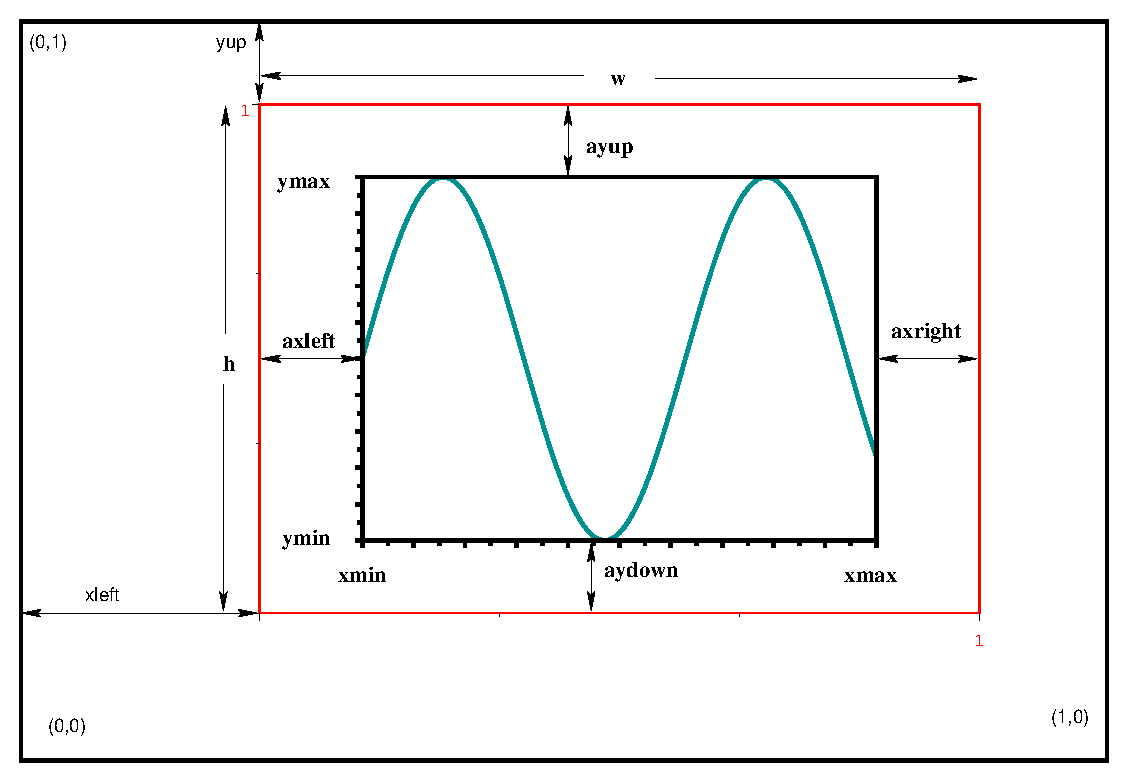
\includegraphics{\mansrc graphics/xsetechfig}
    \end{center}
\end{mandescription}

%--example
\begin{examples}

\noindent two subwindows 

\begin{mintednsp}{nsp}
  xsetech(wrect=[0,0,1.0,0.5],frect=[-5,-3,5,3])
  plot2d([1:10]',[1:10]',style=1,strf="001")
  xsetech(wrect=[0,0.5,1.0,0.5],axesflag=4)
  plot2d([1:10]',[1:10]',strf='014',rect=[-6,-6,6,6]);
\end{mintednsp}

\noindent four subwindows

\begin{mintednsp}{nsp}
  xsetech(wrect=[0,0,0.5,0.5],a3d=%t); plot3d()
  xsetech(wrect=[0.5,0,0.5,0.5]); plot2d()
  xsetech(wrect=[0.5,0.5,0.5,0.5]); grayplot()
  xsetech(wrect=[0,0.5,0.5,0.5]); histplot()
\end{mintednsp}

\noindent using \verb!arect!

\begin{mintednsp}{nsp}
  xsetech(wrect=[0,0,1.0,0.5],arect=1/8*ones(1,4));
  x=1:0.1:10;plot2d(x',sin(x)');
  xsetech(wrect=[0,0.5,1.0,0.5],arect=[2/8,2/8,1/16,1/4]);
  x=1:0.1:10;plot2d(x',sin(x)');
\end{mintednsp}
\end{examples}
%-- see also
\begin{manseealso}
  \manlink{xgetech}{xgetech} \manlink{subplot}{subplot} \manlink{isoview}{isoview} \manlink{square}{square} 
\end{manseealso}
%-- Author

\begin{authors}
  J.-Ph. C.  
\end{authors}


% -*- mode: latex -*-

\mansection{xstring}
\begin{mandesc}
  \short{xstring}{draw a string matrix} \\
  \short{xstringl}{draw a string matrix} \\
\end{mandesc}
%-- Calling sequence section
\begin{calling_sequence}
\begin{verbatim}
  R=xstring(x,y,S,options=value);
  rect=xstringl(x,y,S,options=value);
\end{verbatim}
\end{calling_sequence}
%-- Parameters
\begin{parameters}
  \begin{varlist}
    \vname{x,y}: real scalars, coordinates of a point.
    \vname{S}: a string matrix.
    \vname{angle}: a double, clockwise angle in degree; default is 0.
    \vname{box}: a boolean (default is false).
    \vname{color}: font color.
    \vname{fill}: a boolean.
    \vname{h,w}: two scalar doubles.
    \vname{posx}: a string selected among \verb!'left'!, \verb!'center'!, or \verb!'right'! (default value is \verb!'right'!)
    \vname{posy}: a string selected among \verb!'bottom'!, \verb!'center'!, \verb!'baseline'!, or \verb!'up'! (default value is \verb!'bottom'!).
    \vname{size}: a scalar int giving the font size to use in pixel.
    \vname{R}: a string graphic object
    \vname{rect}: a \verb!1x4! real matrix, \verb![x,y,w,h]!, giving a rectangle coordinates (upper-left point,width,height).
  \end{varlist}
\end{parameters}

\begin{mandescription}
  \verb!xstring! draws the matrix of strings \verb!S! at location \verb!x,y!
  in the current graphic window. Each row of the matrix
  stands for a line of text where row elements are separated by a white space.
  Optional parameters can be given to control the position, size and color of the
  text.

  \begin{description}
  \item[angle]: it gives the slope in degree used for drawing the strings.
    The rotation is around the point \verb!(x,y)! or around the center of the box \verb![x,y,w,h]!
    when  \verb!w! and \verb!h! are given.
  \item[size]: give the font size to use.
  \item[w,h,fill]: when \verb!w! and \verb!h! are given and are not both equal to zero,
    then the string matrix is drawn centered in the box \verb![x,y,w,h]! where
    \verb!(x,y)! is the lower-left point of the box. Then, if \verb!fill! is true
    then the font size is adapter for the string to be contained in the box.
  \item[posx, posy]: The parameters \verb!posx! and \verb!posy! give the relative
    position of the string matrix display from the point \verb!(x,y)!. They can be used
    when \verb!w!, \verb!h! and \verb!fill! are not given.
  \end{description}

  \verb!xstringl! returns a \verb!1x4! matrix giving the coordinates of an enclosing rectangle.

\end{mandescription}

%--example
\begin{examples}

\noindent A first example

  \begin{mintednsp}{nsp}
    xsetech(frect=[0,0,2,2],iso=%t);
    xstring(1,1,["Nsp";"Graphics"])
  \end{mintednsp}

\noindent A second example where the string rotation is around \verb!(x,y)!.

  \begin{mintednsp}{nsp}
    xsetech(frect=[0,0,2,2],iso=%t);
    xset('font size',3);
    for A=[0:30:330];
      x=1+0.5*cos(-%pi*A/180);y=1+0.5*sin(-%pi*A/180);
      xstring(x,y,'Nsp',A,0,color=A/10);
      xsegs([1;x],[1;y]);
    end
  \end{mintednsp}

\noindent A second example where the string rotation is around the center of the
  given box\verb!(x,y,w,h)!.

  \begin{mintednsp}{nsp}
    xsetech(frect=[-1.0,-1.0,1.0,1.0],iso=%t);
    w=0.2,h=0.2;
    for A=[0:30:330];
       x=0.5*cos(-%pi*A/180);y=0.5*sin(-%pi*A/180);
       // (x,y) is upper-left point for xrect
       R=xrect(-w/2,h/2,w,h);
       R.rotate[[cos(-%pi*A/180),sin(-%pi*A/180)]];
       R.translate[[x,y]];
       // (x,y) is lower-left point for xstring
       xstring(x-w/2,y-h/2,'Nsp',fill=%t,w=w,h=h,angle=A,color=A/10);
       xsegs([0;x],[0;y]);
    end
  \end{mintednsp}

\end{examples}

%-- see also
\begin{manseealso}
  \manlink{xnumb}{xnumb} \manlink{xstringb}{xstringb} \manlink{xstringl}{xstringl} \manlink{xtitle}{xtitle}
\end{manseealso}

%-- Author

\begin{authors}
  J.-Ph. C.
\end{authors}

% -*- mode: latex -*-

\mansection{xtitle}
\begin{mandesc}
  \short{xtitle}{sets the main title and the axis labels of a graph}
\end{mandesc}

% -- Calling sequence section
\begin{calling_sequence}
\begin{verbatim}
xtitle(title, [x_title, y_title])
\end{verbatim}
\end{calling_sequence}
% -- Parameters
\begin{parameters}
  \begin{varlist}
    \vname{title}: a matrix of strings. Each line of the matrix corresponds to a new line
    in the title.
    \vname{x_title}: a string corresponding to the label of the x axis
    \vname{y_title}: a string corresponding to the label of the y axis
\end{varlist}
\end{parameters}

\begin{mandescription}
  \verb+xtitle+ adds a title to a graph. \verb+x_title+ and \verb+y_title+ are optional.
\end{mandescription}

\begin{examples}
  \begin{program}
    "x=(1:10)';plot2d(x,x);
    xtitle(['Titre';'Principal'],'x legend ','y legend');"
  \end{program}
\end{examples}

\begin{manseealso}
  plot2d
\end{manseealso}

% -- Authors
\begin{authors}
   jl
\end{authors}


% \input{\mansrc graphics/encours/addcolor.tex}
% \input{\mansrc graphics/encours/alufunctions.tex}
% \input{\mansrc graphics/encours/arc_properties.tex}
% \input{\mansrc graphics/encours/axes_properties.tex}
% \input{\mansrc graphics/encours/axis_properties.tex}
% \input{\mansrc graphics/encours/barhomogenize.tex}
% \input{\mansrc graphics/encours/barh.tex}
% \input{\mansrc graphics/encours/bar.tex}
% \input{\mansrc graphics/encours/black.tex}
% \input{\mansrc graphics/encours/chart.tex}
% \input{\mansrc graphics/encours/clear_pixmap.tex}
% \input{\mansrc graphics/encours/clf.tex}
% \input{\mansrc graphics/encours/colorbar.tex}
% \input{\mansrc graphics/encours/colordef.tex}
% \input{\mansrc graphics/encours/color_list.tex}
% \input{\mansrc graphics/encours/color.tex}
% \input{\mansrc graphics/encours/compound_properties.tex}
% \input{\mansrc graphics/encours/contourf.tex}
% \input{\mansrc graphics/encours/copy.tex}
% \input{\mansrc graphics/encours/delete.tex}
% \input{\mansrc graphics/encours/dragrect.tex}
% \input{\mansrc graphics/encours/drawaxis.tex}
% \input{\mansrc graphics/encours/drawlater.tex}
% \input{\mansrc graphics/encours/drawnow.tex}
% \input{\mansrc graphics/encours/draw.tex}
% \input{\mansrc graphics/encours/driver.tex}
% \input{\mansrc graphics/encours/edit_curv.tex}
% \input{\mansrc graphics/encours/errbar.tex}
% \input{\mansrc graphics/encours/fac3d.tex}
% \input{\mansrc graphics/encours/fchamp.tex}
% \input{\mansrc graphics/encours/fcontour2d.tex}
% \input{\mansrc graphics/encours/fcontour.tex}
% \input{\mansrc graphics/encours/fec_properties.tex}
% \input{\mansrc graphics/encours/fgrayplot.tex}
% \input{\mansrc graphics/encours/figure_properties.tex}
% \input{\mansrc graphics/encours/fplot2d.tex}
% \input{\mansrc graphics/encours/fplot3d1.tex}
% \input{\mansrc graphics/encours/fplot3d.tex}
% \input{\mansrc graphics/encours/gainplot.tex}
% \input{\mansrc graphics/encours/gca.tex}
% \input{\mansrc graphics/encours/gce.tex}
% \input{\mansrc graphics/encours/gcf.tex}
% \input{\mansrc graphics/encours/gda.tex}
% \input{\mansrc graphics/encours/gdf.tex}
% \input{\mansrc graphics/encours/geom3d.tex}
% \input{\mansrc graphics/encours/getcolor.tex}
% \input{\mansrc graphics/encours/getfont.tex}
% \input{\mansrc graphics/encours/getlinestyle.tex}
% \input{\mansrc graphics/encours/getmark.tex}
% \input{\mansrc graphics/encours/getsymbol.tex}
% \input{\mansrc graphics/encours/get.tex}
% \input{\mansrc graphics/encours/GlobalProperty.tex}
% \input{\mansrc graphics/encours/glue.tex}
% \input{\mansrc graphics/encours/graduate.tex}
% \input{\mansrc graphics/encours/graphics_entities.tex}
% \input{\mansrc graphics/encours/Graphics.tex}
% \input{\mansrc graphics/encours/grayplot_properties.tex}
% \input{\mansrc graphics/encours/graypolarplot.tex}
% \input{\mansrc graphics/encours/gr_menu.tex}
% \input{\mansrc graphics/encours/hist3d.tex}
% % -*- mode: latex -*-
% Copyright Lelong 

\mansection{histplot}
\begin{mandesc}
  \short{histplot}{draw an histogram of the components of a vector of numbers}
\end{mandesc}

% -- Calling sequence section
\begin{calling_sequence}
\begin{verbatim}
 histplot(n,data,[normalize=%t|%f,style=val1,rect=val2,axesflag=val3,fill=%t|%f])
 histplot(x,data,[normalize=%t|%f,style=val1,rect=val2,axesflag=val3,fill=%t|%f])
\end{verbatim}
\end{calling_sequence}
% -- Parameters
\begin{parameters}
  \begin{varlist}
    \vname{n}: number of classes for the histogram
    \vname{x}: an increasing vector defining the classes.
    \vname{y}: vector of data.
    \vname{fill}: optional boolean argument, sets whether the bars of the histogram
    should be filled with the color specified by \verb+style+.
    \vname{style=val1}: optional  argument, sets the color of the bars of each
    histogram. \verb+val1+ must be a vector of integers.  When \verb+fill=%f+,
    \verb+style+ sets the color of the contour of each bar.
    \vname{rect=val2}: optional argument, sets the bounds of the plotting
    window. \verb+val2+ must be a vector of integers: \verb+[xmin, ymin, xmax, ymax]+.
    \vname{nax}: not implemented
    \vname{axesflag=val3}: optional argument, specified how axes are
    drown. \verb+val3+ is an integer between \verb+0+ and \verb+5+
    \begin{itemize}
    \item \verb+val3=0+ : no axes are drawn.
    \item \verb+val3=1+ : axes are drawn with the y axis on the left.
    \item \verb+val3=2+ : a box is drawn around the plot.
    \item \verb+val3=3+ : axes are drawn with the y axis on the right.
    \item \verb+val3=4+ : axes are drawn centred in the middle of the plotting window
    \item \verb+val3=5+ : axes are drawn so to cross at the point \verb+(0,0)+.
    \end{itemize}

\end{varlist}
\end{parameters}

\begin{mandescription}
  This function plots an histogram of the vector data using the
  classes x. If \verb+n+ is given, x is defined by x=[min(data):h:max(data)] with
  h=(max(data)-min(data))/n.

  The optional argument \verb+normalise+ (default value \verb+%t+) can be set to
  \verb+%f+.
  optional argument \verb+fill+ (default value \verb+%t+).


  
\end{mandescription}

\begin{examples}
  \begin{program}
    \HCode{g = randn(1,10000);\Hnewline
    histplot(100, g)
    }
  \end{program}

\end{examples}

\begin{manseealso}
  \manlink{xtitle}{xtitle}, \manlink{plot2d}{plot2d}
\end{manseealso}


% \input{\mansrc graphics/encours/hsv2rgb.tex}
% \input{\mansrc graphics/encours/isoview.tex}
% \input{\mansrc graphics/encours/label_properties.tex}
% \input{\mansrc graphics/encours/legend_properties.tex}
% \input{\mansrc graphics/encours/legends.tex}
% \input{\mansrc graphics/encours/legend.tex}
% \input{\mansrc graphics/encours/LineSpec.tex}
% \input{\mansrc graphics/encours/loadplots.tex}
% \input{\mansrc graphics/encours/locate.tex}
% \input{\mansrc graphics/encours/Matplot1.tex}
% \input{\mansrc graphics/encours/Matplot_properties.tex}
% \input{\mansrc graphics/encours/m_circle.tex}
% \input{\mansrc graphics/encours/mesh.tex}
% \input{\mansrc graphics/encours/milk_drop.tex}
% \input{\mansrc graphics/encours/move.tex}
% \input{\mansrc graphics/encours/name2rgb.tex}
% \input{\mansrc graphics/encours/newaxes.tex}
% \input{\mansrc graphics/encours/object_editor.tex}
% \input{\mansrc graphics/encours/oldplot.tex}
% \input{\mansrc graphics/encours/paramfplot2d.tex}
% \input{\mansrc graphics/encours/pie.tex}
% \input{\mansrc graphics/encours/plot2d1.tex}
% \input{\mansrc graphics/encours/plot2d2.tex}
% \input{\mansrc graphics/encours/plot2d3.tex}
% \input{\mansrc graphics/encours/plot2d4.tex}
% \input{\mansrc graphics/encours/plot2d_old_version.tex}
% % -*- mode: latex -*-
% Copyright Lelong 

\mansection{plot2d}
\begin{mandesc}
  \short{plot2d}{draw two dimensional graphs}
\end{mandesc}

% -- Calling sequence section
\begin{calling_sequence}
\begin{verbatim}
plot2d(x,y,[leg=str1, leg_pos=str2, style=val1, rect=val2, axesflag=val3])
\end{verbatim}
\end{calling_sequence}
% -- Parameters
\begin{parameters}
  \begin{varlist}
    \vname{x}: abscissa vector. It can be empty, in this case \verb+[1:length(y)]+ is used.
    \vname{y}: vector or matrix of numbers.
    \vname{style=val1}: optional named argument, sets the style for each curve. \verb+val1+
    must be a vector of integers.
    \vname{rect=val2}: optional named argument, sets the bounds of the plotting
    window. \verb+val2+ must be a vector of integers: \verb+[xmin, ymin, xmax, ymax]+.
    \vname{leg=str1}: optional named argument, str1 must be a string of the form
    \verb+'leg1@leg2@...'+ where \verb+legi+ is the legend associated with the i-th curve.
    \vname{leg_pos=str2}: optional named argument, only useful when \verb+leg=str1+
    is specified. \verb+str2+ is one of these strings ``dr'' (downer right corner), ``ur'' (upper
    right corner), ``dl'' (downer left corner), ``ul'' (upper left corner)
    indicating the position of the legend.
    \vname{axesflag=val3}: optional named argument, specified how axes are
    drown. \verb+val3+ is an integer between \verb+0+ and \verb+5+
    \begin{itemize}
    \item \verb+val3=0+ : no axes are drawn.
    \item \verb+val3=1+ : axes are drawn with the y axis on the left.
    \item \verb+val3=2+ : a box is drawn around the plot.
    \item \verb+val3=3+ : axes are drawn with the y axis on the right.
    \item \verb+val3=4+ : axes are drawn centred in the middle of the plotting window
    \item \verb+val3=5+ : axes are drawn so to cross at the point \verb+(0,0)+.
    \end{itemize}
  \end{varlist}
\end{parameters}

\begin{mandescription}
  plot2d plots a set of two dimensional curves.

  If \verb+y+ is a matrix, each column of \verb+y+ is plotted against vector
  \verb+x+. In this case.

  If \verb+x+ is empty and \verb+y+ is a vector, \verb+plot2d([], y, opt_arg)+ is
  equivalent to \verb|plot2d((1:size(y,'*')), y, opt_arg)|.

  If \verb+x+ is empty and \verb+y+ is a matrix, \verb+plot2d([], y, opt_arg)+ is
  equivalent to \verb|plot2d((1:size(y,'r')), y, opt_arg)|.  
\end{mandescription}

\begin{examples}
  \begin{program}
    \HCode{x=(-\%pi:0.01:\%pi);\Hnewline
    //simple plot\Hnewline
    plot2d(x, sin(x));\Hnewline
\Hnewline
    //multiple plot\Hnewline
    plot2d(x, [sin(x)', cos(x)'], leg='sin@cos', style=[3,4], leg_pos='ul');\Hnewline
\Hnewline
    x=(-3:0.01:3)\Hnewline
    xtitle('density of the normal distribution')\Hnewline
    plot2d(x, exp(-x.*x/2)/sqrt(2*\%pi), rect=[-3,0,3,1]);
    }
  \end{program}
\end{examples}

\begin{manseealso}
  \manlink{xtitle}{xtitle}
\end{manseealso}

% -- Authors

% \input{\mansrc graphics/encours/plot3d1.tex}
% \input{\mansrc graphics/encours/plot3d2.tex}
% \input{\mansrc graphics/encours/plot3d3.tex}
% \input{\mansrc graphics/encours/plot3d_old_version.tex}
% % -*- mode: latex -*-
\mansection{plot3d}
\begin{mandesc}
  \short{plot3d}{3D plot of a surface}\\
  \short{plot3d1}{3D plot of a surface}\\
\end{mandesc}
% -- Calling sequence section
\begin{calling_sequence}
\begin{verbatim}
  plot3d(x,y,z,args=,alpha=,colormap=,colors=,ebox=,
         flag=,leg=,theta=,mesh=,mesh_only=,shade=);

  plot3d(x,y,f,args=,alpha=,colormap=,colors=,ebox=,
         flag=,leg=,theta=,mesh=,mesh_only=,shade=);
\end{verbatim}
\end{calling_sequence}

%-- Parameters
\begin{parameters}
  \begin{varlist}
    \vname{x,y,z} first possible case: \verb!x! and \verb!y! can be vectors of
    respective size \verb!n1! and \verb!n2! and in that case they give x-axis
    and y-axis coordinates of the surface and \verb!z! must be a matrix of size
    \verb!n1 x n2!.  \verb!z(i,j)! is the value of the surface at the point
    (x(i),y(j)).
    %
    \vname{x,y,z} second possible case: \verb!x! and \verb!y! and \verb!z!  are
    matrices of size \verb!nf x n!.  In that case, they define the \verb!n!
    facets which compose the surface. The i-th gacet is defined by a polygon
    with \verb!nf! points.  The coordinates of the points of the i-th facet are
    given respectively by \verb!xf(:,i)!, \verb!yf(:,i)! and \verb!zf(:,i)!.
    %
    \vname{colors}: a vector of size \verb!n! giving the color of each facets or
    a matrix of size \verb!nf x n! giving color at each facet extreme
    points. Facet colors are then interpolated or averaged depending on the
    optional \verb!shade! parameter.
    %
    \vname{theta, alpha}: optional arguments giving in degree the spherical coordinates of the
    observation point.
    %
    \vname{leg}: optional string defining the labels for each axis with \verb!@! as a field
    separator, for example \verb!"X@Y@Z"!.
    %
    \vname{flag}: optional real vector of size three.
    \verb!flag=[mode,type,box]!.
    \begin{varlist}
      \vname{mode}: an integer (surface color).
      \begin{varlist}
        \vname{mode$>$0}: the surface is painted with color
        \verb!"mode"! ; the boundary of the facet is drawn
        with current line style and color.\vname{mode=0:}a mesh of the surface is drawn.
        \vname{mode$<$0:}the surface is painted with color \verb!"-mode"! ; the boundary of the facet is not
        drawn.
      \end{varlist}
      \vname{type}: an integer (scaling).
      \begin{varlist}
        \vname{type=0}: the plot is made using the current 3D scaling.
        \vname{type=1}: rescales automatically 3d boxes with extreme aspect
        ratios, the boundaries are specified by the value of the
        optional argument \verb!ebox!.
        \vname{type=2}: rescales automatically 3d boxes with extreme aspect
        ratios, the boundaries are computed using the given
        data.
        \vname{type=3}: 3d isometric with box bounds given by optional \verb!ebox!, similarily to
        \verb!type=1!.
        \vname{type=4}: 3d isometric bounds derived from the data, similarily tp \verb!type=2!.
        \vname{type=5}: 3d expanded isometric bounds with box bounds given by optional \verb!ebox!, similarily to
        \verb!type=1!.
        \vname{type=6}: 3d expanded isometric bounds derived from the data,
        similarily to \verb!type=2!.
      \end{varlist}
      \vname{box}: an integer (frame around the plot).
      \begin{varlist}
        \vname{box=0}: nothing is drawn around the plot.
        \vname{box=1}: unimplemented (like box=0).
        \vname{box=2}: only the axes behind the surface are drawn.
        \vname{box=3}: a box surrounding the surface is drawn and captions are added.
        \vname{box=4}: a box surrounding the surface is drawn, captions and
        axes are added.
      \end{varlist}
    \end{varlist}
    %
    \vname{ebox}: vector \verb![xmin,xmax,ymin,ymax,zmin,zmax]! used to fix the
    boundaries of the plot. This argument is used when the optional argument
    \verb!flag! is given with type set to \verb!1!, or \verb!3!, or \verb!5!.
    \vname{mesh}: a boolean specifying if the mesh is to be drawn.
    \vname{mesh_only}: a boolean specifying if only the mesh is to be drawn.
  \end{varlist}
\end{parameters}

\begin{mandescription}
  When \verb!x! and \verb!y! are vectors of respective size \verb!n1! and
  \verb!n2! and \verb!z! is a matrix of size \verb!n1 x n2!  a parametric
  surface which value $z(i,j)$ at point $(x(i),y(j)$ is drawn.  holes can be
  inserted in the surface by setting some values to \verb!%nan!.

  When \verb!x!, \verb!y!, and \verb!z! are matrices of the same size. They
  describe a set of facets which are drawn.  In that case, specific color for
  each facet can be given through the optional parameter \verb!color!.

  When \verb!plot3d1! is used instead of \verb!plot3d!, z-values are mapped to
  colors of the current colormap.
\end{mandescription}
%--example
\begin{examples}

\noindent a first simple example with \verb!plot3d!

\begin{mintednsp}{nsp}
  t=-%pi:0.3:%pi;plot3d(t,t,sin(t)'*cos(t));
\end{mintednsp}

\noindent a first simple example with \verb!plot3d1! (the default
colormap is a jetcolormap).

\begin{mintednsp}{nsp}
  t=-%pi:0.3:%pi;plot3d1(t,t,sin(t)'*cos(t));
\end{mintednsp}

\noindent same example with mesh only

\begin{mintednsp}{nsp}
  t=-%pi:0.3:%pi;plot3d(t,t,sin(t)'*cos(t),mesh_only=%t);
\end{mintednsp}

\noindent same example without mesh

\begin{mintednsp}{nsp}
  t=-%pi:0.3:%pi;plot3d(t,t,sin(t)'*cos(t),mesh=%f);
\end{mintednsp}

\noindent same example with a function

\begin{mintednsp}{nsp}
  function z=f(x,y,args) z=sin(args(1)*x)*cos(args(2)*y);endfunction;
  // the optional argument arg is used to pass extra arguments to function f.
  t=-%pi:0.3:%pi;plot3d(t,t,f,args=list(1,2));
\end{mintednsp}

\noindent computing facets and plot facets with colors

\begin{mintednsp}{nsp}
  t=-%pi:0.3:%pi;
  z=sin(t)'*cos(t);
  [xx,yy,zz]=genfac3d(t,t,z);
  plot3d(xx,yy,zz,colors=linspace(1,40,400),colormap=hotcolormap(40));
  // remode shade i.e one color per face
  xclear();
  plot3d(xx,yy,zz,colors=linspace(1,40,400),colormap=hotcolormap(40),shade=%f);
\end{mintednsp}

multiple plots by combining facets

\begin{mintednsp}{nsp}
  t=-%pi:0.3:%pi;
  z=sin(t)'*cos(t);
  [xx,yy,zz]=genfac3d(t,t,z);
  z=sin(2*t)'*cos(t);
  [m,n]=size(xx);
  [xx1,yy1,zz1]=genfac3d(t,t,z);
  plot3d([xx,xx1],[yy,yy1],[zz,zz1],colors=[20*ones(1,n),30*ones(1,n)],colormap=hotcolormap(40));
\end{mintednsp}

multiple plots using opengl

\begin{mintednsp}{nsp}
  xinit(opengl=%t);
  z=sin(t)'*cos(t);
  [xx,yy,zz]=genfac3d(t,t,z);
  [m,n]=size(xx);
  plot3d(xx,yy,zz,colors=[20*ones(1,n)],colormap=hotcolormap(40));
  z=sin(2*t)'*cos(t);
  [xx,yy,zz]=genfac3d(t,t,z);
  plot3d(xx,yy,zz,colors=[30*ones(1,n)],colormap=hotcolormap(40));
\end{mintednsp}
\end{examples}

%-- see also
\begin{manseealso}
  \manlink{eval3dp}{eval3dp} \manlink{genfac3d}{genfac3d} \manlink{geom3d}{geom3d}
  \manlink{param3d}{param3d} \manlink{plot3d1}{plot3d1} \manlink{fec}{fec}
  \manlink{xdel}{xdel}
\end{manseealso}

%-- Author

\begin{authors}
  J.Ph.C and B. Pin�on
\end{authors}

% \input{\mansrc graphics/encours/plotframe.tex}
% \input{\mansrc graphics/encours/plot.tex}
% \input{\mansrc graphics/encours/plzr.tex}
% \input{\mansrc graphics/encours/polyline_properties.tex}
% \input{\mansrc graphics/encours/printing.tex}
% \input{\mansrc graphics/encours/rectangle_properties.tex}
% \input{\mansrc graphics/encours/replot.tex}
% \input{\mansrc graphics/encours/rgb2name.tex}
% \input{\mansrc graphics/encours/rotate.tex}
% \input{\mansrc graphics/encours/rubberbox.tex}
% \input{\mansrc graphics/encours/scaling.tex}
% \input{\mansrc graphics/encours/sca.tex}
% \input{\mansrc graphics/encours/scf.tex}
% \input{\mansrc graphics/encours/sd2sci.tex}
% \input{\mansrc graphics/encours/sda.tex}
% \input{\mansrc graphics/encours/sdf.tex}
% \input{\mansrc graphics/encours/secto3d.tex}
% \input{\mansrc graphics/encours/segs_properties.tex}
% \input{\mansrc graphics/encours/set_posfig_dim.tex}
% \input{\mansrc graphics/encours/set.tex}
% \input{\mansrc graphics/encours/sgrid.tex}
% \input{\mansrc graphics/encours/show_pixmap.tex}
% \input{\mansrc graphics/encours/square.tex}
% \input{\mansrc graphics/encours/stringbox.tex}
% \input{\mansrc graphics/encours/surface_properties.tex}
% \input{\mansrc graphics/encours/surf.tex}
% \input{\mansrc graphics/encours/text_properties.tex}
% \input{\mansrc graphics/encours/titlepage.tex}
% \input{\mansrc graphics/encours/title.tex}
% \input{\mansrc graphics/encours/twinkle.tex}
% \input{\mansrc graphics/encours/unglue.tex}
% \input{\mansrc graphics/encours/unzoom.tex}
% \input{\mansrc graphics/encours/xaxis.tex}
% \input{\mansrc graphics/encours/xbasc.tex}
% \input{\mansrc graphics/encours/xbasimp.tex}
% \input{\mansrc graphics/encours/xbasr.tex}
% \input{\mansrc graphics/encours/xchange.tex}
% \input{\mansrc graphics/encours/xclea.tex}
% \input{\mansrc graphics/encours/xclick.tex}
% \input{\mansrc graphics/encours/xclip.tex}
% % -*- mode: latex -*-
\mansection{xdel}
\begin{mandesc}
  \short{xdel}{delete a graphics window}\\ 
\end{mandesc}
%-- Calling sequence section
\begin{calling_sequence}
\begin{verbatim}
  xdel([winsid])   
\end{verbatim}
\end{calling_sequence}
%-- Parameters
\begin{parameters}
  \begin{varlist}
    \vname{winid}: integer or integer vector\end{varlist}
\end{parameters}
\begin{mandescription}
  The function \verb!xdel! deletes the graphics windows whose id are given by 
  \verb!winsid! or delete the current graphics window if no argument is given.
\end{mandescription}
%-- Author
\begin{authors}
  J.-Ph. C.  
\end{authors}


% \input{\mansrc graphics/encours/xend.tex}
% % -*- mode: latex -*-

\mansection{xfarcs}
\begin{mandesc}
  \short{xfarcs}{fill parts of a set of ellipses}\\ % @mandesc@
\end{mandesc}
%-- Calling sequence section
\begin{calling_sequence}
\begin{verbatim}
  R=xfarcs(rects,[colors])
  R=xfarcs(rects,color=..,thickness=..,background=..,compound=%t|%f);
\end{verbatim}
\end{calling_sequence}

%-- Parameters
\begin{parameters}
  \begin{varlist}
    \vname{arcs}: matrix of size (6,n) describing the ellipses.
    \vname{colors}: row vector of size n.
    \vname{background}: vector of size n.
    \vname{color}: vector of size n.
    \vname{thickness}: vector of size n.
    \vname{compound}: a boolean.
    \vname{R}: a graphic object.
  \end{varlist}
\end{parameters}

\begin{mandescription}
  \verb!xfarcs! fills parts of a set of ellipses described by \verb!arcs!: 
  \verb!arcs=[x y w h a1 a2;x y w h a1 a2;...]'! where each ellipse is defined 
  by the 6 parameters \verb!(x,y,w,h,a1,a2)! (see \verb!xarc!).
  The value of \verb!colors(i)! gives the color to use for filling ellpise \verb!i!.

  \verb!xfarcs(arcs,color=..,thickness=..,background=..,compound=%t|%f);! 
  draws parts of a set of ellipses. The color and thickness of drawing line can be given by optional arguments
  color and thickness. If optional background argument is given it is used as color to fill
  the rectangle. A graphic object is returned in argument \verb!R! if requested and by default
  its is a compound which contains all the graphics rectangle objects.
\end{mandescription}

%--example
\begin{examples}
  \begin{mintednsp}{nsp}
    xsetech(frect=[-1,-1,1,1]);
    arcs=[-1.0 0.0 0.5; // upper left x
           1.0 0.0 0.5; // upper left y
           0.5 1.0 0.5; // width
           0.5 0.5 1.0; // height
           0.0 0.0 0.0; // angle 1
           180*64 360*64 90*64]; // angle 2
    xfarcs(arcs,color=[1,2,3],thickness=[3,3,3],background=[-2,5,6])
  \end{mintednsp}
\end{examples}

%-- see also
\begin{manseealso}
  \manlink{xarc}{xarc} \manlink{xfarc}{xfarc} \manlink{xfarcs}{xarcs} 
\end{manseealso}

%-- Author

\begin{authors}
  J.-Ph. C.;   
\end{authors}


% % -*- mode: latex -*-
\mansection{xfarc}
\begin{mandesc}
  \short{xfarc}{fill a part of an ellipse}\\ % @mandesc@
\end{mandesc}
%-- Calling sequence section
\begin{calling_sequence}
\begin{verbatim}
  A=xfarc(x,y,w,h,a1,a2,options=value)
  A=xfarc(arc,options=value)
\end{verbatim}
\end{calling_sequence}
%-- Parameters
\begin{parameters}
  \begin{varlist}
    \vname{x,y,w,h}: four real values defining a rectangle.
    \vname{a1,a2}: real values defining a sector.
    \vname{arc}: a vector of size \verb!6! 
    \vname{background, color, thickness}: optional arguments.
    \vname{A}: a graphical rectangle object.
  \end{varlist}
\end{parameters}

\begin{mandescription}
  \verb!xfarc! fills a part of an ellipse contained in the rectangle 
  \verb!(x,y,w,h)!
  (upper-left point, width, height), and in the sector defined by 
  the angle \verb!alpha1! and the angle \verb!alpha1+alpha2!. 
  \verb!alpha1! and \verb!alpha2! are 
  given respectively by \verb!a1/64! degrees and \verb!a2/64! degrees.
  This function uses the current color and graphics scale.

  The color and thickness of drawing line can be given by optional arguments
  \verb!color! and \verb!thickness!. If optional \verb!background!
  argument is given it is used as color to fill the rectangle.

  If \verb!color! is positive it gives the color to be used for drawing,
  if \verb!color=-1! the default color is used, if  \verb!color=-2! the
  rectangle is not drawn.

  If \verb!background! is positive it gives the color to be used for filling,
  if \verb!background=-1! the default filling color is used,
  if  \verb!background=-2! the rectangle is not filled.
  
\end{mandescription}

%--example
\begin{examples}
  \begin{mintednsp}{nsp}
    xsetech(frect=[-2,-2,2,2],iso=%t,axesflag=0);
    xfarc(-1,1,2,2,0,90*64,background=7,color=3);
    xarc(-1.5,1.5,3,3,0,360*64)
  \end{mintednsp}
\end{examples}

%-- see also
\begin{manseealso}
  \manlink{xarc}{xarc} \manlink{xarcs}{xarcs} \manlink{xfarcs}{xfarcs} 
\end{manseealso}

%-- Author

\begin{authors}
  J.Ph.C.;   

\end{authors}


% % -*- mode: latex -*-

\mansection{xfpolys}
\begin{mandesc}
  \short{xfpolys}{fill a set of polygons}\\ % @mandesc@
\end{mandesc}
%-- Calling sequence section
\begin{calling_sequence}
\begin{verbatim}
  A=xfpolys(xpols,ypols,fill,options=value)
  A=xfpolys(xpols,ypols,options=value)
\end{verbatim}
\end{calling_sequence}

%-- Parameters
\begin{parameters}
  \begin{varlist}
    \vname{xpols,ypols}: two real matrices of size \verb!pxn!.
    \vname{fill}: vector of size \verb!n! or of size \verb!pxn!.
    \vname{A}: if requested \verb!A! is a graphic polyline object or a graphic compound object.
    \vname{color}: a scalar or a vector of size \verb!n!
    \vname{compound}: a boolean  specifying if returned value is a compound or the last polyline.
    \vname{fill_color}: a scalar or a vector of size \verb!n!
    \vname{thickness}:  a scalar or a vector of size \verb!n!
  \end{varlist}
\end{parameters}

\begin{mandescription}
  \verb!xfpolys! fills with colors a set of polygons of the same size defined by
  the two matrices \verb!xpols! and \verb!ypols!. The coordinates of the points of the
  \verb!i!-th polygon are given by columns \verb!i! of \verb!xpols! and \verb!ypols!.

  % The polygons may be filled with a given color (flat) or painted with
  % interpolated (shaded) colors.

  % \begin{description}
  % \item[flat color painting] In this case \verb!fill! should be a vector of size
  %   \verb!n!. The color to be used for filling polygon number \verb!i! is given by \verb!fill(i)!:
  %   \begin{description}
  %   \item[-] if \verb!fill(i)$<$0!, the polygon is filled with color \verb!-fill(i)!.
  %   \item[-] if \verb!fill(i)=0!, the polygon is drawn with the current color) and not filled.
  %   \item[-] if \verb!fill(i)$>$0!, the polygon is filled with color \verb!fill(i)! and
  %     the boundary is drawn with the current color.
  %   \end{description}
  % \item[interpolated color painting]
  %   In this case \verb!fill! should be a matrix with same sizes
  %   as \verb!xpols! and \verb!ypols!. Note that
  %   \verb!p! must be equal to 3 or 4.
  %   \verb!fill(k,i)! gives the color at the \verb!k!th edge
  %   of polygon \verb!i!.
  % \end{description}

  The argument \verb!fill! is used to specify the colors to be used for drawing and filling polygons
  The vector \verb!fill! should be a vector of size \verb!n! and the color to be used for filling
  polygon number \verb!i! is given by \verb!fill(i)!:
  \begin{description}
  \item[-] if \verb!fill(i)$<$0!, the polygon is filled with color \verb!-fill(i)!.
  \item[-] if \verb!fill(i)=0!, the polygon is drawn with the current color) and not filled.
  \item[-] if \verb!fill(i)$>$0!, the polygon is filled with color \verb!fill(i)! and
    the boundary is drawn with the current color.
  \end{description}

  The colors for drawing the boundaries and filling the polygons can also be given by
  optional named parameters. Negative values for some optional named parameters like \verb!color! or
  \verb!fill_color! have special meaning. Parameters are ignored when they are equal to \verb!-2!
  and are set to default values if they are equal to \verb!-1!.
\end{mandescription}

%--example
\begin{examples}

\noindent Using a \verb!fill! argument
\begin{mintednsp}{nsp}
  xsetech(frect=[-10,-10,210,40]);
  x1=[0,10,20,30,20,10,0]';
  y1=[15,30,30,15,0,0,15]';
  xpols=[x1 x1 x1 x1]; xpols=xpols+[0,60,120,180].*.ones(size(x1));
  ypols=[y1 y1 y1 y1];
  xset('thickness',3);
  xfpolys(xpols,ypols,[-1,0,10,13])
\end{mintednsp}

\noindent Using options

\begin{mintednsp}{nsp}
  xsetech(frect=[-10,-10,210,40]);
  x1=[0,10,20,30,20,10,0]';
  y1=[15,30,30,15,0,0,15]';
  xpols=[x1 x1 x1 x1]; xpols=xpols+[0,60,120,180].*.ones(size(x1));
  ypols=[y1 y1 y1 y1];
  xfpolys(xpols,ypols,color=[-2,-1,5,6], fill_color=[4,-2,10,13],thickness=3);
\end{mintednsp}

\noindent Mixing \verb!plot2d! and \verb!xfpolys!

\begin{mintednsp}{nsp}
function plot2d_polys(x,y,n,s,varargopt)
  plot2d(x,y,varargopt(:));
  z=ones(1,size(x,'*'));
  p=[x(:)';y(:)'];
  qx=p;qy=p;
  for i=1:n
    qx(i,:)=p(1,:)+s/2*cos(2*%pi*i/n);
    qy(i,:)=p(2,:)+s/2*sin(2*%pi*i/n);
  end
  v.fill_color= z* varargopt.find['line_color',def=-1];
  v.color=z;
  xfpolys(qx,qy,v(:));
endfunction

x=1:20;y=x.*sin(x);plot2d_polys(x,y/3,5,1.0,line_color=5)
\end{mintednsp}

\end{examples}

%-- see also
\begin{manseealso}
  \manlink{xfpoly}{xfpoly} \manlink{xpoly}{xpoly} \manlink{xpolys}{xpolys}
\end{manseealso}

%-- Author

\begin{authors}
  J.Ph.C.

\end{authors}

% % -*- mode: latex -*-
\mansection{xfpoly}
\begin{mandesc}
  \short{xfpoly}{fill a polygon with color}\\
\end{mandesc}
% -- Calling sequence section
\begin{calling_sequence}
\begin{verbatim}
  p=xfpoly(x,y,fill_color=,color=,thickness)
\end{verbatim}
\end{calling_sequence}
%-- Parameters
\begin{parameters}
  \begin{varlist}
    \vname{x,y}: two real vectors of same size \verb!pxn!.
    \vname{color}: color to be used for drawing boundary (default \verb!-2!).
    \vname{fill_color}: color for filling the polyline (default \verb!-1!).
    \vname{thickness}: thickness of boundary (default \verb!-1!).
    \vname{p}: a graphics polyline object.
  \end{varlist}
\end{parameters}

\begin{mandescription}
  \verb!xfpoly! fills a polygon with color and draws the boundary of
  the polygon if color is not equal to \verb!-2!.

  Negative values for some parameters have special meaning.
  Parameters are ignored when they are equal to \verb!-2!
  and are set to default values if they are equal to \verb!-1!.
\end{mandescription}

%--example
\begin{examples}
  \begin{mintednsp}{nsp}
    x=sin(2*%pi*(0:4)/5);
    y=cos(2*%pi*(0:4)/5);
    xsetech(frect=[-2,-2,2,2])
    xfpoly(x,y,color=6,fill_color=4,thickness=3);
  \end{mintednsp}
\end{examples}

%-- see also
\begin{manseealso}
  \manlink{xfpolys}{xfpolys} \manlink{xpoly}{xpoly} \manlink{xpolys}{xpolys}
\end{manseealso}

%-- Author

\begin{authors}
  J.Ph.C.

\end{authors}

% \input{\mansrc graphics/encours/xgetech.tex}
% \input{\mansrc graphics/encours/xgetmouse.tex}
% \input{\mansrc graphics/encours/xget.tex}
% \input{\mansrc graphics/encours/xgraduate.tex}
% \input{\mansrc graphics/encours/xgrid.tex}
% \input{\mansrc graphics/encours/xinfo.tex}
% \input{\mansrc graphics/encours/xinit.tex}
% \input{\mansrc graphics/encours/xlfont.tex}
% \input{\mansrc graphics/encours/xload.tex}
% \input{\mansrc graphics/encours/xname.tex}
% % -*- mode: latex -*-

\mansection{xnumb}
\begin{mandesc}
  \short{xnumb}{draw numbers}\\ % @mandesc@
\end{mandesc}
%-- Calling sequence section
\begin{calling_sequence}
\begin{verbatim}
  xnumb(x,y,nums,[box,angle])  
\end{verbatim}
\end{calling_sequence}

%-- Parameters
\begin{parameters}
  \begin{varlist}
    \vname{x,y,nums}: vectors of same size.\vname{box}: integer value.\vname{angle}: optional vector of same size as \verb!x!\end{varlist}
\end{parameters}

\begin{mandescription}
  \verb!xnumb! draws the value of \verb!nums(i)!
  at position \verb!x(i),y(i)! in the current scale.
  If \verb!box! is 1, a box is drawn around the numbers. 
  If \verb!angle! is given, it gives the direction for string drawing.
\end{mandescription}

%--example
\begin{examples}
  \begin{mintednsp}{nsp}
    xsetech(frect=[-100,-100,500,600]);
    x=0:100:200;
    xnumb(x,500*ones(size(x)),[10,20,35],1)
  \end{mintednsp}
\end{examples}
%-- see also
\begin{manseealso}
  \manlink{xstring}{xstring} 
\end{manseealso}
%-- Author

\begin{authors}
  J.-Ph. C.  
\end{authors}


% % -*- mode: latex -*-
\mansection{xpause}
\begin{mandesc}
  \short{xpause}{pause execution of nsp}\\
\end{mandesc}
%-- Calling sequence section
\begin{calling_sequence}
\begin{verbatim}
  xpause(d [,events])
\end{verbatim}
\end{calling_sequence}
\begin{parameters}
  \begin{varlist}
    \vname{d} a real scalar for the pause duration in microseconds.
    \vname{events}: an optional boolean parameter
  \end{varlist}
\end{parameters}
%
\begin{mandescription}
  The function \verb!xpause! pauses the current process for
  a duration of \verb!d!-microseconds. If the second argument
  is given and set to \verb!%t! then Gtk events are processed
  during the pause. When the duration is set to \verb!0! pending
  events are also processed.
\end{mandescription}
%-- Author
\begin{authors}
  J.-Ph. C.
\end{authors}

% \input{\mansrc graphics/encours/xrpoly.tex}
% \input{\mansrc graphics/encours/xs2bmp.tex}
% \input{\mansrc graphics/encours/xs2emf.tex}
% \input{\mansrc graphics/encours/xs2eps.tex}
% \input{\mansrc graphics/encours/xs2fig.tex}
% \input{\mansrc graphics/encours/xs2gif.tex}
% \input{\mansrc graphics/encours/xs2ppm.tex}
% \input{\mansrc graphics/encours/xs2ps.tex}
% \input{\mansrc graphics/encours/xsave.tex}
% \input{\mansrc graphics/encours/xsetm.tex}
% \input{\mansrc graphics/encours/xset.tex}
% \input{\mansrc graphics/encours/xstringb.tex}
% % -*- mode: latex -*-

\mansection{xstring}
\begin{mandesc}
  \short{xstring}{draw a string matrix} \\
  \short{xstringl}{draw a string matrix} \\
\end{mandesc}
%-- Calling sequence section
\begin{calling_sequence}
\begin{verbatim}
  R=xstring(x,y,S,options=value);
  rect=xstringl(x,y,S,options=value);
\end{verbatim}
\end{calling_sequence}
%-- Parameters
\begin{parameters}
  \begin{varlist}
    \vname{x,y}: real scalars, coordinates of a point.
    \vname{S}: a string matrix.
    \vname{angle}: a double, clockwise angle in degree; default is 0.
    \vname{box}: a boolean (default is false).
    \vname{color}: font color.
    \vname{fill}: a boolean.
    \vname{h,w}: two scalar doubles.
    \vname{posx}: a string selected among \verb!'left'!, \verb!'center'!, or \verb!'right'! (default value is \verb!'right'!)
    \vname{posy}: a string selected among \verb!'bottom'!, \verb!'center'!, \verb!'baseline'!, or \verb!'up'! (default value is \verb!'bottom'!).
    \vname{size}: a scalar int giving the font size to use in pixel.
    \vname{R}: a string graphic object
    \vname{rect}: a \verb!1x4! real matrix, \verb![x,y,w,h]!, giving a rectangle coordinates (upper-left point,width,height).
  \end{varlist}
\end{parameters}

\begin{mandescription}
  \verb!xstring! draws the matrix of strings \verb!S! at location \verb!x,y!
  in the current graphic window. Each row of the matrix
  stands for a line of text where row elements are separated by a white space.
  Optional parameters can be given to control the position, size and color of the
  text.

  \begin{description}
  \item[angle]: it gives the slope in degree used for drawing the strings.
    The rotation is around the point \verb!(x,y)! or around the center of the box \verb![x,y,w,h]!
    when  \verb!w! and \verb!h! are given.
  \item[size]: give the font size to use.
  \item[w,h,fill]: when \verb!w! and \verb!h! are given and are not both equal to zero,
    then the string matrix is drawn centered in the box \verb![x,y,w,h]! where
    \verb!(x,y)! is the lower-left point of the box. Then, if \verb!fill! is true
    then the font size is adapter for the string to be contained in the box.
  \item[posx, posy]: The parameters \verb!posx! and \verb!posy! give the relative
    position of the string matrix display from the point \verb!(x,y)!. They can be used
    when \verb!w!, \verb!h! and \verb!fill! are not given.
  \end{description}

  \verb!xstringl! returns a \verb!1x4! matrix giving the coordinates of an enclosing rectangle.

\end{mandescription}

%--example
\begin{examples}

\noindent A first example

  \begin{mintednsp}{nsp}
    xsetech(frect=[0,0,2,2],iso=%t);
    xstring(1,1,["Nsp";"Graphics"])
  \end{mintednsp}

\noindent A second example where the string rotation is around \verb!(x,y)!.

  \begin{mintednsp}{nsp}
    xsetech(frect=[0,0,2,2],iso=%t);
    xset('font size',3);
    for A=[0:30:330];
      x=1+0.5*cos(-%pi*A/180);y=1+0.5*sin(-%pi*A/180);
      xstring(x,y,'Nsp',A,0,color=A/10);
      xsegs([1;x],[1;y]);
    end
  \end{mintednsp}

\noindent A second example where the string rotation is around the center of the
  given box\verb!(x,y,w,h)!.

  \begin{mintednsp}{nsp}
    xsetech(frect=[-1.0,-1.0,1.0,1.0],iso=%t);
    w=0.2,h=0.2;
    for A=[0:30:330];
       x=0.5*cos(-%pi*A/180);y=0.5*sin(-%pi*A/180);
       // (x,y) is upper-left point for xrect
       R=xrect(-w/2,h/2,w,h);
       R.rotate[[cos(-%pi*A/180),sin(-%pi*A/180)]];
       R.translate[[x,y]];
       // (x,y) is lower-left point for xstring
       xstring(x-w/2,y-h/2,'Nsp',fill=%t,w=w,h=h,angle=A,color=A/10);
       xsegs([0;x],[0;y]);
    end
  \end{mintednsp}

\end{examples}

%-- see also
\begin{manseealso}
  \manlink{xnumb}{xnumb} \manlink{xstringb}{xstringb} \manlink{xstringl}{xstringl} \manlink{xtitle}{xtitle}
\end{manseealso}

%-- Author

\begin{authors}
  J.-Ph. C.
\end{authors}

% \input{\mansrc graphics/encours/xtape.tex}
% % -*- mode: latex -*-

\mansection{xtitle}
\begin{mandesc}
  \short{xtitle}{sets the main title and the axis labels of a graph}
\end{mandesc}

% -- Calling sequence section
\begin{calling_sequence}
\begin{verbatim}
xtitle(title, [x_title, y_title])
\end{verbatim}
\end{calling_sequence}
% -- Parameters
\begin{parameters}
  \begin{varlist}
    \vname{title}: a matrix of strings. Each line of the matrix corresponds to a new line
    in the title.
    \vname{x_title}: a string corresponding to the label of the x axis
    \vname{y_title}: a string corresponding to the label of the y axis
\end{varlist}
\end{parameters}

\begin{mandescription}
  \verb+xtitle+ adds a title to a graph. \verb+x_title+ and \verb+y_title+ are optional.
\end{mandescription}

\begin{examples}
  \begin{program}
    "x=(1:10)';plot2d(x,x);
    xtitle(['Titre';'Principal'],'x legend ','y legend');"
  \end{program}
\end{examples}

\begin{manseealso}
  plot2d
\end{manseealso}

% -- Authors
\begin{authors}
   jl
\end{authors}

% \input{\mansrc graphics/encours/zgrid.tex}
% \input{\mansrc graphics/encours/zoom_rect.tex}
